
\documentclass[12pt]{report}

% language may be romanian or english (default is english)
% type may be bachelor or master (default is bachelor)
\usepackage[language=english, type=bachelor]{style}

\usepackage{amsmath,amssymb,mathtools}
\usepackage{booktabs}
\usepackage{tabularx}
\usepackage{array}
\usepackage{float}
\usepackage{caption}
\usepackage{subcaption}
\usepackage{enumitem}
\usepackage[table]{xcolor}
\usepackage{fancyhdr}
\usepackage{longtable}
\usepackage{multirow}
\usepackage{rotating}
\usepackage{microtype}
\usepackage{ragged2e}
\usepackage{xurl}
\graphicspath{{./}}

\pagestyle{fancy}
\fancyhf{}
\lhead{}
\chead{}
\rhead{\thepage}
\cfoot{\thepage}
\renewcommand{\headrulewidth}{0.2pt}
\renewcommand{\footrulewidth}{0pt}
\setlength{\headheight}{15pt}
\fancypagestyle{plain}{%
  \fancyhf{}
  \fancyhead[R]{\thepage}
  \fancyfoot[C]{\thepage}
  \renewcommand{\headrulewidth}{0.2pt}
  \renewcommand{\footrulewidth}{0pt}
}

\hypersetup{
    colorlinks=true,
    linkcolor=black,
    citecolor=black,
    urlcolor=blue,
    pdftitle={Neural Decoding of Visual Perception from fMRI Using CLIP-Guided Generative Models},
    pdfauthor={Iepure Antoniu}
}

\setlength{\parskip}{0.35em}
\setlength{\parindent}{1.2em}
\setlist[itemize]{leftmargin=1.6em}
\renewcommand{\arraystretch}{1.2}
\captionsetup{font=small,labelfont=bf}
\renewcommand{\bibname}{Bibliography}

% Project-specific tokens like SHARED1000 and N1v28a contain digits and
% therefore cannot be added to \hyphenation{...} (LaTeX rejects non-letter
% tokens there).  Allow looser inter-word spacing instead so the paragraph
% breaker has room to avoid the overfull boxes those long tokens otherwise
% cause at the right margin.
\emergencystretch=3em
\tolerance=1000
\hbadness=2000

\newcommand{\placeholderfigure}[3]{%
\begin{figure}[htbp]
    \centering
    \fcolorbox{black}{gray!10}{%
        \begin{minipage}[c][#1][c]{0.84\textwidth}
            \centering
            {\Large \textbf{Figure Placeholder}}\\[0.5em]
            \emph{#2}\\[0.4em]
            Insert the final exported image here after the experiments are completed.\\[0.3em]
            {\small Source: author placeholder.}
        \end{minipage}}
    \caption{#2}
    \label{#3}
\end{figure}}

\begin{document}

\specialization{Artificial Intelligence}
\specializationRO{Inteligen\c t\u a Artificial\u a}
\title{Neural Decoding of Visual Perception from fMRI\\Using CLIP-Guided Generative Models}
\titleRO{Decodificarea neural\u a a percep\c tiei vizuale din fMRI\\folosind modele generative ghidate de CLIP}
\author{Iepure Antoniu}
\supervisor{Prof. univ. dr. Anca-Mirela Andreica}

\maketitle
\pagenumbering{roman}

\chapter*{Abstract}
\addcontentsline{toc}{chapter}{Abstract}

This bachelor thesis studies neural decoding of visual perception from functional magnetic resonance imaging (fMRI) by learning a mapping from 7T brain activity in the Natural Scenes Dataset to CLIP-aligned image representations. The thesis is retrieval-first: instead of predicting pixels directly, the proposed framework predicts image-aligned latent variables that are better suited to nearest-neighbour retrieval and to controlled downstream generation. The main contribution is a reproducible decoding pipeline in which compact retrieval, shortlist-local reranking, rich latent regression, and frozen score-level expert fusion are treated as distinct but cooperative components. The final exported system combines three independently trained retrieval experts---a 197k-token-space model with 16-draw Monte Carlo test-time augmentation and two complementary 768-D experts---and reaches $86.3\%$ CSLS Recall@1 on the held-out SHARED1000 benchmark. A secondary SDXL~1.0 + IP-Adapter reconstruction add-on, conditioned on the retrieved top-1 image and an fMRI-predicted CLIP signal, yields modest improvements in SSIM, PSNR, CLIP image similarity, and AlexNet(5)-level identification on $141$ SHARED1000 examples, while leaving pixel correlation, LPIPS, and early AlexNet features essentially unchanged. Retrieval is the main quantitative contribution of the thesis; the reconstruction module is anchor-dependent and should not be interpreted as a pure fMRI-only reconstruction.

\textbf{Keywords:} fMRI, neural decoding, CLIP, diffusion models, retrieval, NSD.

\tableofcontents
\newpage
\pagenumbering{arabic}


\chapter{Introduction}
\label{chap:introduction}

Recovering visual information from brain activity is one of the most ambitious goals of modern computational neuroscience. In recent years, large-scale neuroimaging datasets, multimodal representation learning, and generative models have enabled a shift from coarse category decoding toward image-specific retrieval and plausible visual reconstruction from fMRI signals \cite{Allen2022,Ozcelik2023,Scotti2023,Scotti2024}. This progress is scientifically important because it connects two difficult problems: understanding how the visual cortex represents semantic and structural information, and learning machine representations that can act as bridges between biological measurements and natural images.

The present thesis focuses on the \emph{visual perception} setting. During each trial, a subject observes a natural image and the corresponding blood-oxygen-level-dependent (BOLD) response is recorded with high-field fMRI. The central task is to infer an image-aligned latent representation from this neural signal. Rather than predicting pixels directly, the pipeline maps fMRI activity into a CLIP-based embedding space, where similarity can be measured reliably and where downstream diffusion-based image generation becomes possible \cite{Radford2021,Rombach2022}. This choice turns the problem into a structured latent prediction task rather than a fragile direct image regression problem.

Formally, let $x_i \in \mathbb{R}^{V}$ denote the preprocessed voxel vector for trial $i$, where $V$ is the number of selected voxels, and let $z_i \in \mathbb{R}^{d}$ denote the target image embedding extracted from a pretrained vision-language model. The decoder is a parametric mapping
\begin{equation}
\hat{z}_i = f_{\theta}(x_i), \qquad f_{\theta}: \mathbb{R}^{V} \rightarrow \mathbb{R}^{d},
\label{eq:intro_mapping}
\end{equation}
where $\hat{z}_i$ should preserve enough image-specific information to retrieve the correct image from a held-out gallery and, later, to condition a generative model. The main evaluation scenario is therefore retrieval: for each predicted embedding, the system searches a gallery of candidate images and ideally ranks the ground-truth item first.

This formulation is challenging for several reasons. First, fMRI is an indirect and noisy measurement of neural activity, with low temporal resolution and substantial inter-session variability \cite{Allen2022,Wen2018}. Second, the representation space of modern visual models is high-dimensional and geometrically nontrivial \cite{Radford2021,Conneau2018}. Third, there is a constant risk of data leakage or protocol mismatch when repeated images, subject-specific preprocessing, and cached features are involved. A strong bachelor thesis in this area must therefore be both algorithmically ambitious and experimentally rigorous.

The main research question of this thesis is the following: \emph{how can one learn a stable mapping from cortical activity to an image-aligned latent space that supports accurate retrieval and provides a credible foundation for visual reconstruction?} The project approaches this question through an iterative experimental program. Early stages establish robust baselines and eliminate implementation errors. Later stages explore probabilistic decoders, directional losses, richer targets, multi-head retrieval designs, and shortlist-based fusion strategies.

\section{Motivation and Context}

The work is motivated by the convergence of three research directions. The first is the availability of datasets such as the Natural Scenes Dataset, which provide image-level behavioural and neuroimaging data at a scale that was previously unavailable \cite{Allen2022}. The second is the emergence of CLIP-style multimodal latent spaces, which align image representations with semantic structure and perform well in retrieval settings \cite{Radford2021}. The third is the success of latent diffusion models, which make it possible to turn recovered latent information into realistic image samples \cite{Rombach2022,Ozcelik2023,Takagi2023}. Together, these directions make fMRI-to-image decoding both more realistic and more measurable than in earlier generations of brain-decoding systems.

\begin{figure}[htbp]
    \centering
    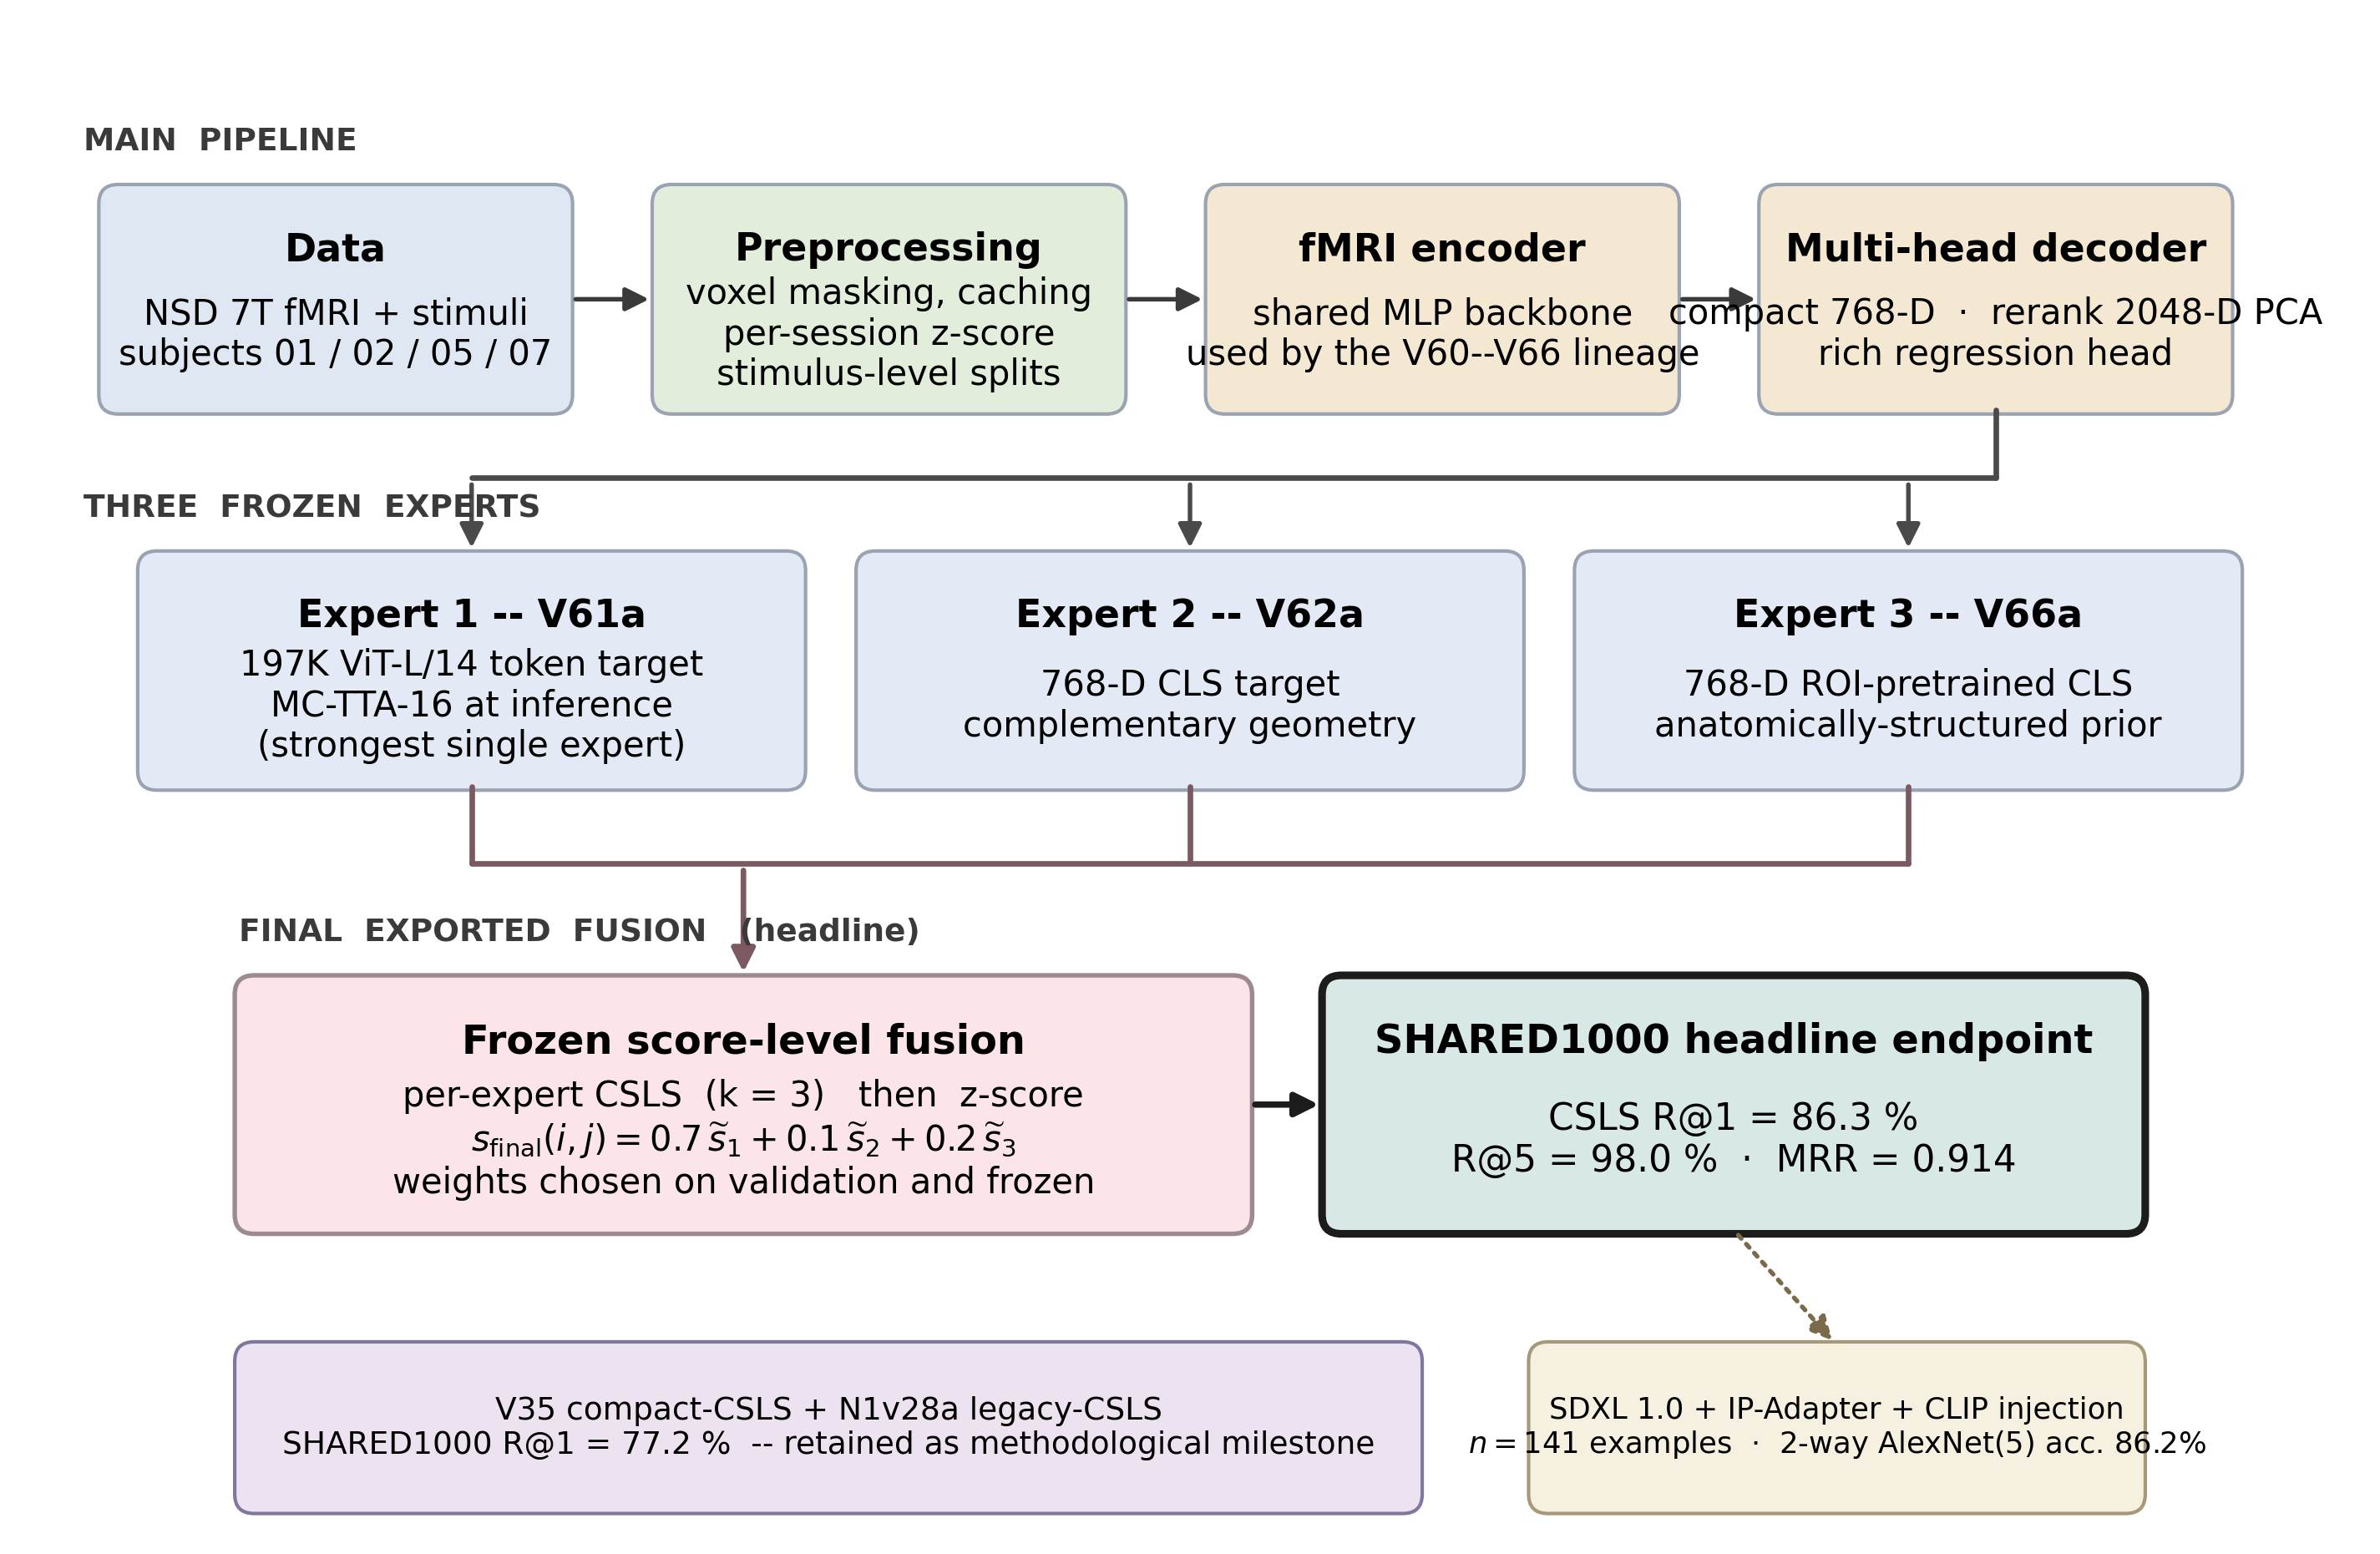
\includegraphics[width=\textwidth]{thesis_pipeline.png}
    \caption{Overview of the complete thesis pipeline. The written thesis is centered on retrieval: NSD fMRI is preprocessed and mapped by a shared encoder into compact, rerank, and rich latent heads. The V35 plus frozen legacy N1v28a fixed fusion is retained as a methodological milestone, while the final exported system is a frozen cross-architecture triple score fusion that combines a 197K token-space model with MC-TTA, a 768-D CLS model, and a 768-D ROI-pretrained model. The diffusion add-on is treated as an optional qualitative extension rather than as the primary benchmark.}
    \label{fig:thesis_pipeline}
\end{figure}

A complementary single-example view is useful because it makes the retrieval-first logic concrete. Starting from one viewed stimulus and its matched cortical response, the thesis builds a CLIP target embedding from the image, learns a brain-to-latent mapping from the associated fMRI activity, and then evaluates the predicted latent first through held-out retrieval and only secondarily through optional qualitative generation.

\begin{figure}[htbp]
    \centering
    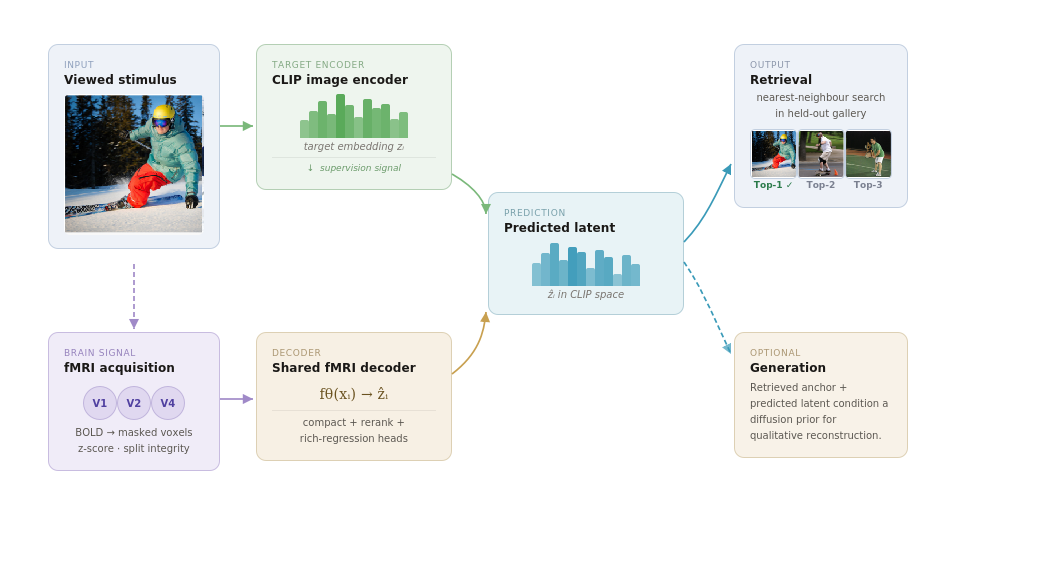
\includegraphics[width=0.94\textwidth]{end_to_end_example_pipeline.png}
    \caption{Single-example decoding path used throughout the thesis. A viewed image defines the target CLIP embedding, the corresponding fMRI response is preprocessed into a voxel vector, and the decoder learns to map that brain activity into the shared latent space used for retrieval-first evaluation and optional downstream generation.}
    \label{fig:end_to_end_example_pipeline}
\end{figure}

\section{Objectives of the Thesis}

The thesis has four concrete objectives:
\begin{itemize}
    \item to construct a reproducible pipeline for mapping fMRI activity to CLIP-aligned visual embeddings;
    \item to evaluate how architectural and loss-design choices affect retrieval quality under a leakage-free protocol;
    \item to analyse why some experimentally attractive ideas fail, especially under hubness and representation-geometry constraints;
    \item to validate a multi-stage retrieval strategy in which compact retrieval, dedicated reranking, and frozen score-level fusion across complementary experts are treated as distinct but cooperative inference mechanisms.
\end{itemize}

These objectives are intentionally both scientific and engineering-oriented. The final artifact is not only a set of metric values, but also a structured experimental framework in which preprocessing, target caching, training, evaluation, qualitative analysis, and implementation validation are integrated into a single research pipeline.

\section{Original Contributions of the Author}

The original contributions emphasized in this thesis are the following:
\begin{itemize}
    \item the design and implementation of an end-to-end fMRI-to-latent decoding pipeline built around NSD, CLIP targets, and retrieval-based evaluation;
    \item a systematic debugging and validation program addressing alignment, split integrity, checkpoint selection, and retrieval geometry;
    \item an experimental comparison between single-head, dual-head, and triple-head retrieval formulations under a shared protocol;
    \item the validation of shortlist-local reranking as a corrective mechanism, followed by a stronger frozen fixed-fusion milestone built on the V35 compact expert and the legacy N1v28a expert, and finally extended into a frozen cross-architecture triple score fusion that combines a 197K token-space model with MC-TTA and two complementary 768-D experts as the final exported retrieval system;
    \item a conservative qualitative analysis of retrieval-guided diffusion refinement, showing where anchor-preserving generation is useful and where exact retrieval should remain unchanged;
    \item the explicit documentation of negative results and failed directions, which is scientifically useful because it narrows future search space.
\end{itemize}

At the time of writing, the work has not yet been presented as a peer-reviewed conference publication. The thesis therefore serves as the primary written record of the experimental results, methodological design, and implementation choices.

\section{Transparency Regarding the Use of Generative AI Tools}

In accordance with the university guidelines, the author states transparently that generative AI tools were used only in a limited and assistive manner during the preparation of the manuscript. Their use was restricted to language polishing, reformulation suggestions, and LaTeX refactoring support. The scientific content, literature verification, experimental design, software implementation, numerical results, and interpretation of findings remain the full responsibility of the author. No generative AI system is treated as an author or as an authoritative source of scientific truth.

\section{Structure of the Thesis}

The remainder of the thesis is organized as follows. Chapter~\ref{chap:background} reviews the theoretical background, the relevant literature, the historical evolution of the field, the NSD dataset, and the main evaluation metrics used in the project. Chapter~\ref{chap:methodology} presents the proposed methodology, including preprocessing, target construction, model design, and the multi-head retrieval formulation. Chapter~\ref{chap:implementation} describes the software design, experiment management, validation strategy, and reproducibility measures of the implemented system. Chapter~\ref{chap:experiments} reports the experimental evolution of the project, summarizes the main results, and discusses their scientific interpretation. Finally, Chapter~\ref{chap:conclusions} summarizes the conclusions, limitations, and future directions.


\chapter{Theoretical Background and Related Work}
\label{chap:background}

\section{Domain and Subdomain of the Thesis}

The thesis belongs to the broad domain of artificial intelligence applied to computational neuroscience. More specifically, it is situated at the intersection of brain decoding, representation learning, and generative modelling. The subdomain addressed here is \emph{visual perception decoding from fMRI}: given a measured cortical response, the goal is to recover information about the external image stimulus that produced it. This task differs from classical neuroimaging analysis because it is not limited to identifying which brain regions are active; instead, it seeks to infer \emph{what was seen} by mapping neural activity into a meaningful computational representation \cite{Kay2008,Naselaris2009}.

\section{Historical Evolution of Visual Decoding}

Visual decoding from fMRI has progressed from low-level stimulus recovery to semantically rich latent reconstruction. Early work showed that activation patterns in the visual cortex carry enough information to infer image structure and to identify natural images and naturalistic scenes \cite{Thirion2006,Kay2008,Naselaris2009,Nishimoto2011}. Subsequent work moved to deep-feature decoding and generative reconstruction with GANs and large CNN features \cite{Horikawa2017,Wen2018,Seeliger2018,Shen2019,VanRullen2019}, and the most recent phase relies on multimodal latent spaces and strong generative priors: latent-diffusion reconstructions \cite{Takagi2023,Ozcelik2023}, contrastive retrieval-plus-reconstruction frameworks (MindEye \cite{Scotti2023}), and shared-subject scaling (MindEye2 \cite{Scotti2024}). The present thesis belongs to this recent phase and emphasises retrieval-oriented latent decoding.

\section{fMRI-Based Visual Decoding}

Functional magnetic resonance imaging measures the BOLD signal, which acts as an indirect proxy for neural activity \cite{Allen2022,Wen2018}. In visual decoding tasks, the input is usually a voxel vector derived from one or more regions of interest in the visual cortex, while the target corresponds to some representation of the viewed stimulus. Earlier approaches focused on category labels or hand-crafted image descriptors \cite{Thirion2006,Kay2008,Naselaris2009}. More recent work predicts features from deep visual models, which allows the decoder to preserve semantic and structural information at a much richer level \cite{Horikawa2017,Wen2018,Scotti2023}.

Let $x_i \in \mathbb{R}^{V}$ be the voxel vector for trial $i$. A basic decoder predicts $\hat{z}_i \in \mathbb{R}^{d}$, where $z_i$ is the target visual representation extracted from the ground-truth image. Because the embedding space is usually normalized, cosine similarity becomes the natural scoring function:
\begin{equation}
\cos(\hat{z}_i, z_j) = \frac{\hat{z}_i^{\top} z_j}{\lVert \hat{z}_i \rVert_2 \, \lVert z_j \rVert_2}.
\label{eq:cosine_similarity}
\end{equation}
A retrieval system ranks all gallery items according to this similarity and checks whether the correct image is recovered near the top of the list.

\section{Natural Scenes Dataset}

The Natural Scenes Dataset is one of the most important benchmarks for high-resolution visual decoding from fMRI \cite{Allen2022}. It contains 7T fMRI responses recorded while subjects viewed thousands of natural images. The scale, signal quality, and repeated-image structure of NSD make it especially suitable for studying image-specific decoding. However, NSD also imposes strict requirements on data handling: repeated trials, image identifiers, train/validation separation, and session-level normalization must all be treated carefully to avoid leakage.

In this thesis, the practical role of NSD is twofold. First, it provides the paired $(x_i, z_i)$ examples needed for supervised learning. Second, it offers a benchmark environment in which the quality of retrieval and reconstruction can be discussed relative to recent systems such as MindEye and MindEye2 \cite{Scotti2023,Scotti2024}. The present work does not attempt to replace NSD-specific discipline with ad hoc experimentation; on the contrary, it treats split integrity and reproducibility as first-class methodological requirements.

\begin{figure}[htbp]
    \centering
    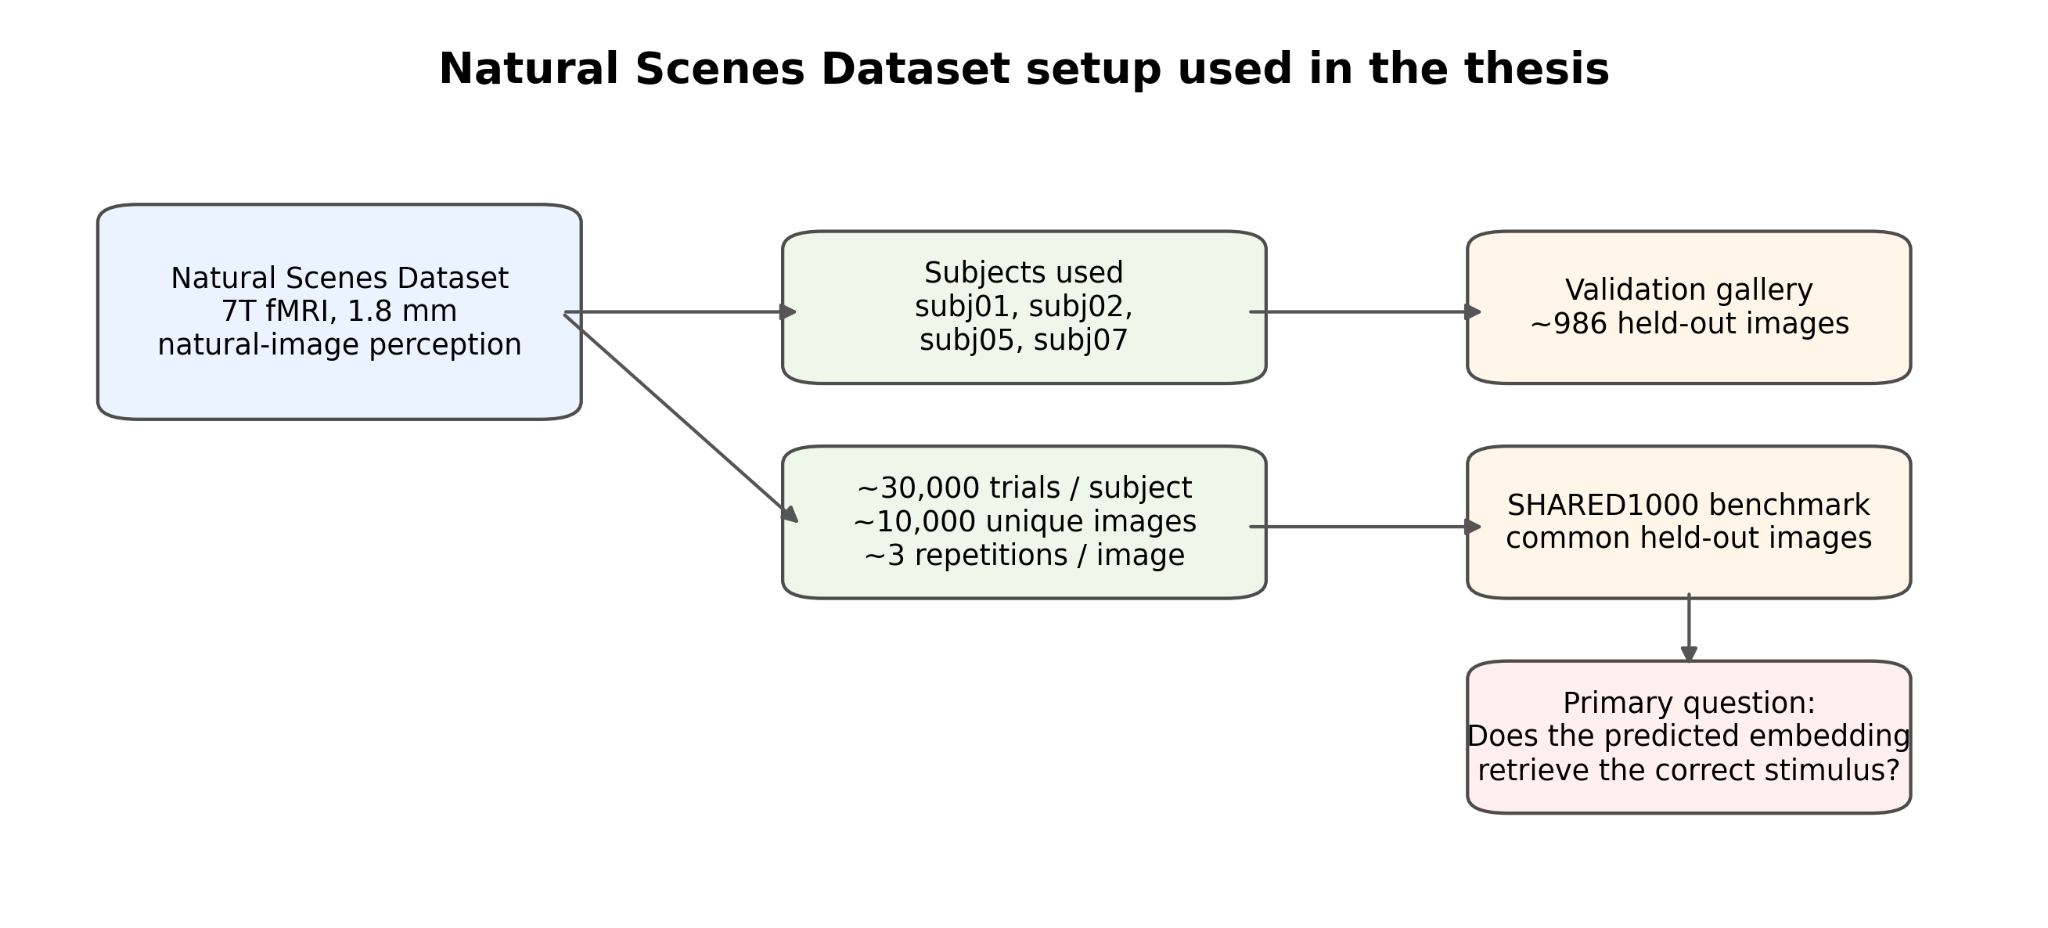
\includegraphics[width=0.96\textwidth]{nsd_overview.png}
    \caption{Dataset setting used throughout the thesis. The work is developed on the Natural Scenes Dataset under a retrieval-oriented protocol, with validation and SHARED1000 treated as the main endpoints.}
    \label{fig:nsd_overview}
\end{figure}

\section{CLIP as the Target Representation}

CLIP learns a shared representation space for images and text using large-scale contrastive supervision \cite{Radford2021}. Its image encoder produces embeddings that are semantically meaningful, well structured for nearest-neighbour search, and highly reusable across downstream tasks. For brain decoding, CLIP is useful because it provides a target space that is already organized around visual-semantic similarity.

This thesis uses CLIP-style image embeddings as latent targets instead of direct pixel supervision. The practical benefit is that the decoder does not need to reconstruct raw images directly from noisy brain signals. Instead, it predicts a representation that can support both retrieval and conditioning of a downstream generator. This idea aligns well with recent diffusion-based reconstruction pipelines \cite{Takagi2023,Ozcelik2023,Scotti2023}.

Figure~\ref{fig:clip_shared_space_alignment} illustrates the geometric intuition behind this choice. CLIP places semantically corresponding images and text descriptions in neighboring regions of a shared embedding space. In the present thesis, this shared geometry becomes the decoding target: a predicted brain embedding is useful only insofar as it lands near the correct image neighborhood while remaining separated from semantically plausible distractors.

\begin{figure}[htbp]
    \centering
    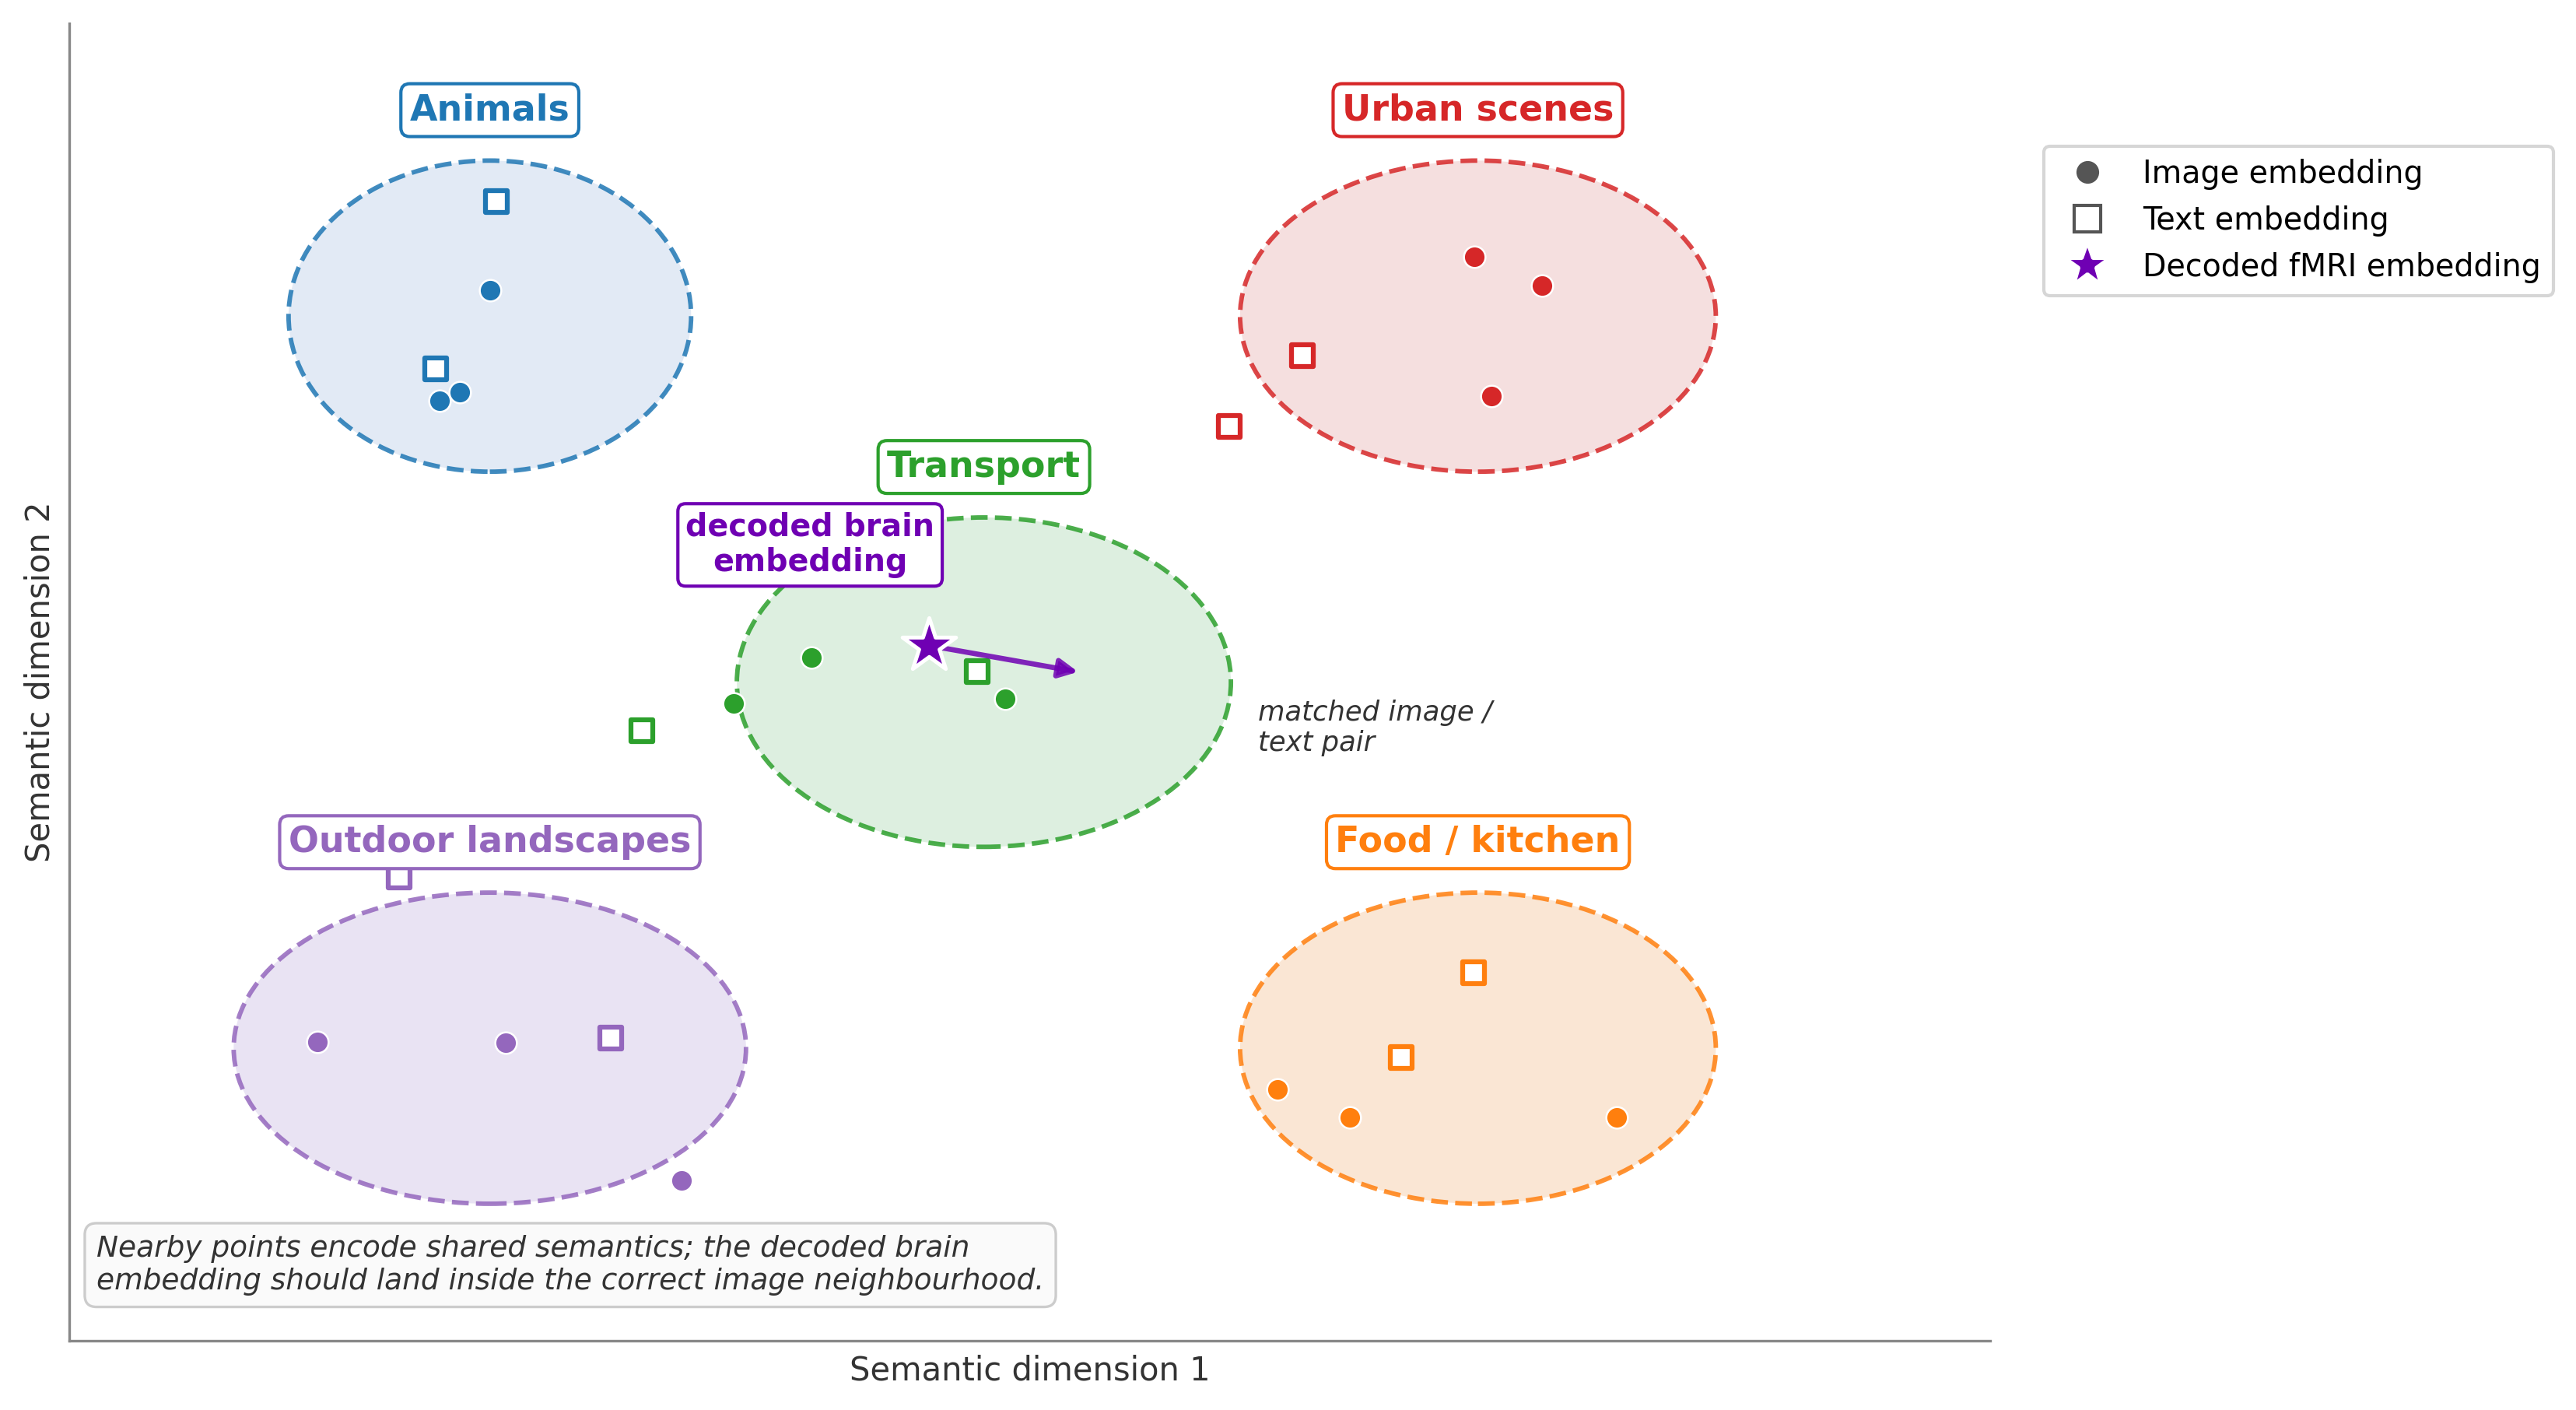
\includegraphics[width=0.96\textwidth]{clip_shared_space_alignment.png}
    \caption{Conceptual view of CLIP as a shared semantic space. Image and text embeddings for related concepts occupy nearby regions, which is why CLIP provides a meaningful target geometry for brain decoding and retrieval.}
    \label{fig:clip_shared_space_alignment}
\end{figure}

\section{Latent Diffusion Models and Generative Reconstruction}

Latent diffusion models synthesize images by iteratively denoising a latent variable conditioned on text, image, or other contextual information \cite{Rombach2022}. A forward step perturbs a clean latent $y_0$ as
\begin{equation}
y_t \sim \mathcal{N}\!\left(\sqrt{1-\beta_t}\, y_{t-1},\, \beta_t I\right),
\label{eq:diffusion_forward}
\end{equation}
and the learned reverse process recovers a clean latent conditioned on the predicted visual representation \cite{Takagi2023,Ozcelik2023}. In this thesis, reconstruction is a downstream extension; retrieval remains the main quantitative focus.

\section{Retrieval Geometry and Hubness}

Accurate latent regression is not sufficient by itself; what matters quantitatively is the geometry of the predicted embeddings relative to the gallery. High-dimensional retrieval spaces suffer from \emph{hubness}: a few gallery items become nearest neighbours for an excessive number of queries, distorting raw cosine retrieval and making a model appear less discriminative than its regression error would suggest \cite{Conneau2018}. The project therefore relies on hubness-aware scoring; the resulting distinction between latent fidelity and retrieval geometry is one of the key interpretive lessons of the experiments.

\section{Evaluation Metrics}

The core metric used throughout the thesis is Recall@K. For a predicted embedding $\hat{z}_i$ and a gallery $\mathcal{G}$, Recall@K is defined as
\begin{equation}
\mathrm{R@K} = \frac{1}{N} \sum_{i=1}^{N} \mathbf{1}\left[\operatorname{rank}(g_i^\star \mid \hat{z}_i) \leq K\right],
\label{eq:recall_at_k}
\end{equation}
where $g_i^\star$ is the ground-truth gallery image corresponding to sample $i$. In this thesis, Recall@1 is the most important endpoint because it directly measures image-specific identification.

A second important metric is cross-domain similarity local scaling (CSLS), which corrects for hubness in high-dimensional retrieval spaces \cite{Conneau2018}. Let $r_q(\hat{z}_i)$ denote the average similarity between query $\hat{z}_i$ and its $k$ nearest gallery neighbours, and let $r_g(z_j)$ denote the average similarity between gallery item $z_j$ and its $k$ nearest query neighbours. Then CSLS is defined as
\begin{equation}
\mathrm{CSLS}(\hat{z}_i, z_j) = 2\,\cos(\hat{z}_i, z_j) - r_q(\hat{z}_i) - r_g(z_j).
\label{eq:csls}
\end{equation}
CSLS is particularly relevant in the present project because the experiments repeatedly show that raw regression fidelity and retrieval geometry are not the same thing.

For the reconstruction add-on the thesis additionally reports the image-fidelity scores standard in this literature \cite{Scotti2023,Scotti2024,Ozcelik2023}: pixel correlation, SSIM, PSNR, LPIPS, CLIP image similarity, and feature-space cosine similarity at two depths of an ImageNet-pretrained AlexNet. Following MindEye and Brain Diffuser, AlexNet(2) uses second-block activations (early texture/edge features) and AlexNet(5) uses fifth-block activations (mid-level, more semantically organized features); all activations are flattened and $\ell_2$-normalized before the cosine product. These metrics are auxiliary, not retrieval endpoints. Reconstruction is reported on $141$ SHARED1000 examples, with AlexNet 2-way identification reported over the $137$ non-perfect cases (excluding the perfect bucket, where the comparison is degenerate).

\section{Representative Related Work}

Recent fMRI-to-image decoding has converged on learned latent representations conditioned on strong generative priors \cite{Ozcelik2023,Takagi2023} or paired with contrastive retrieval and shared-subject scaling \cite{Scotti2023,Scotti2024}. Three lessons from this body of work directly motivate the present methodology: (i) target representation quality matters substantially, with richer embeddings often outperforming simpler regression targets; (ii) data scale and subject alignment remain the dominant practical bottlenecks; and (iii) retrieval and generation are best treated as related but distinct objectives.

\begin{table}[htbp]
\centering
\small
\begin{tabularx}{\textwidth}{>{\raggedright\arraybackslash}p{2.7cm} >{\raggedright\arraybackslash}p{2.6cm} >{\raggedright\arraybackslash}p{3.2cm} >{\raggedright\arraybackslash}X}
\toprule
\textbf{Work} & \textbf{Main idea} & \textbf{Representation / generator} & \textbf{Relevance to this thesis} \\
\midrule
Allen et al. (2022) \cite{Allen2022} & Large-scale 7T benchmark dataset & NSD data resource & Provides the experimental foundation and evaluation setting \\
Radford et al. (2021) \cite{Radford2021} & Vision-language contrastive pretraining & CLIP embedding space & Supplies the latent target space used for decoding \\
Takagi and Nishimoto (2023) \cite{Takagi2023} & Stable-Diffusion-based reconstruction & Latent diffusion conditioning & Shows how strong pretrained generators can be coupled with decoded features \\
Ozcelik and VanRullen (2023) \cite{Ozcelik2023} & Generative latent diffusion for natural scenes & Brain-to-latent diffusion conditioning & Motivates the reconstruction pathway after latent decoding \\
Scotti et al. (2023) \cite{Scotti2023} & Contrastive fMRI-to-image retrieval and reconstruction & CLIP-style targets and diffusion prior & Directly inspires the retrieval-oriented framing of the present work \\
Scotti et al. (2024) \cite{Scotti2024} & Shared-subject scaling for fMRI-to-image decoding & Shared-subject alignment and modern retrieval design & Serves as an upper benchmark and clarifies the role of scale and alignment \\
\bottomrule
\end{tabularx}
\caption{Representative works most closely related to the thesis topic.}
\label{tab:related_work}
\end{table}



\chapter{Proposed Methodology}
\label{chap:methodology}

\section{Problem Formulation}

The thesis addresses supervised neural decoding in the perception setting. Each training example consists of a pair $(x_i, z_i)$, where $x_i$ is the preprocessed fMRI feature vector and $z_i$ is a target image representation extracted from the corresponding viewed stimulus. The learning objective is to estimate a decoder $f_{\theta}$ such that the predicted representation
\begin{equation}
\hat{z}_i = f_{\theta}(x_i)
\label{eq:decoder_prediction}
\end{equation}
is close to the correct target and sufficiently discriminative relative to all other targets in the gallery.

In practice, the decoder does not solve a single homogeneous problem. The later stages of the thesis distinguish between three complementary roles: compact retrieval, reranking, and rich regression. This leads naturally to a multi-head architecture,
\begin{equation}
\big(\hat{z}^{(c)}_i, \hat{z}^{(r)}_i, \hat{z}^{(g)}_i\big) = f_{\theta}(x_i),
\label{eq:multihead_decoder}
\end{equation}
where the superscripts denote the compact head, rerank head, and rich generative/regression head, respectively.

\section{Data Preparation and Preprocessing}

The preprocessing pipeline transforms raw NSD-derived activity into model-ready vectors. The core steps are voxel selection, repeated-trial aggregation when needed, subject/session indexing, per-session normalization, and alignment with image identifiers and cached visual targets. A crucial principle throughout the project is that train/validation separation must occur at the image level, not merely at the trial level, so that repeated observations of the same image do not leak across splits \cite{Allen2022}.

If $x_{i,s}$ denotes the feature vector for sample $i$ in session $s$, z-scoring is performed using statistics estimated only from the training data of that session:
\begin{equation}
\tilde{x}_{i,s} = \frac{x_{i,s} - \mu_s^{\mathrm{train}}}{\sigma_s^{\mathrm{train}} + \varepsilon}.
\label{eq:zscore}
\end{equation}
This reduces session-specific drift while preserving discriminative variation relevant to decoding. In practical terms, the preprocessing stage is not a mere data-cleaning step; it is part of the scientific method, because even a strong architecture becomes meaningless if the split logic or target lookup is incorrect.

\begin{figure}[htbp]
    \centering
    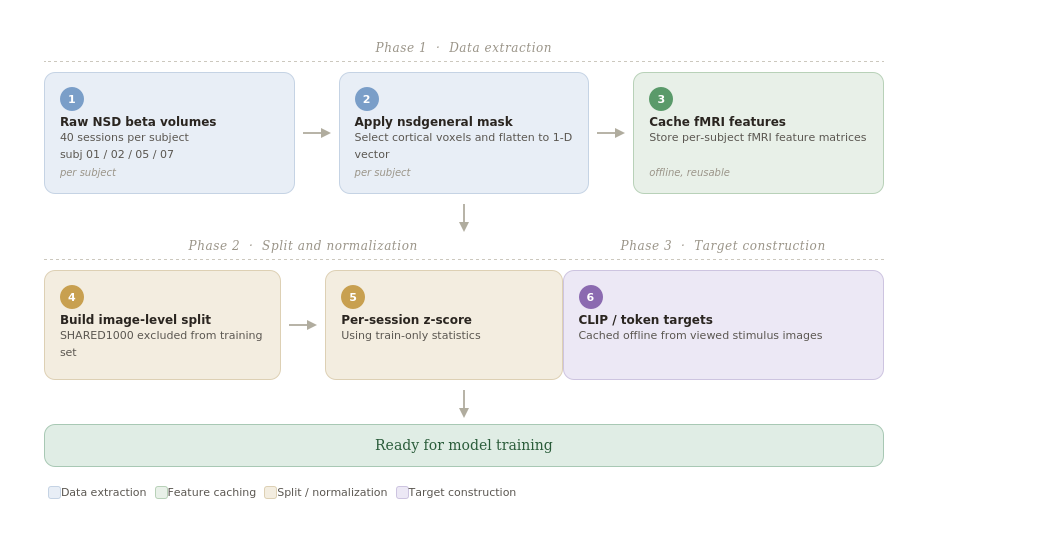
\includegraphics[width=\textwidth]{preprocessing_pipeline.png}
    \caption{Preprocessing and target-construction workflow used in the thesis. The pipeline emphasizes offline caching, image-level split integrity, and per-session normalization before model training.}
    \label{fig:preprocessing_pipeline}
\end{figure}

\section{Latent Targets}

The primary targets are CLIP image embeddings or derived token-level variants obtained from the viewed stimulus image. Let $\phi(I_i)$ denote the target representation extracted from image $I_i$ by a pretrained visual model. The simplest pooled-target formulation uses
\begin{equation}
 z_i = \phi(I_i) \in \mathbb{R}^{d},
\label{eq:target_embedding}
\end{equation}
while richer variants preserve token-level or multi-scale structure. The experiments reported in the thesis show that target quality and granularity have a large effect on retrieval performance, especially when the decoder is strong enough to exploit that additional information \cite{Radford2021,Scotti2023}.

In the methodological evolution of the project, target design became one of the decisive axes of improvement. Compact pooled targets are easier to optimize for shortlist retrieval, whereas richer targets preserve more semantic and structural information for downstream regression and generative reconstruction. The final system therefore treats target richness as a design choice rather than as a universally monotone improvement.

\section{Training Objectives}

The compact head is primarily optimized for ranking. A standard contrastive formulation is the InfoNCE loss \cite{Oord2018}:
\begin{equation}
\mathcal{L}_{\mathrm{NCE}} = -\frac{1}{N}\sum_{i=1}^{N}
\log
\frac{\exp\left(\cos(\hat{z}^{(c)}_i, z_i)/\tau\right)}
{\sum_{j=1}^{N} \exp\left(\cos(\hat{z}^{(c)}_i, z_j)/\tau\right)}.
\label{eq:info_nce}
\end{equation}
Here $\tau > 0$ is a temperature hyperparameter controlling the sharpness of the ranking distribution.

Some experiments model the predicted latent direction probabilistically through a von Mises--Fisher (vMF) output, a natural choice for unit-norm directional embeddings \cite{Banerjee2005}. If $\mu_i$ is a unit-norm mean direction and $\kappa_i$ is a concentration parameter, the density of the target direction can be written as
\begin{equation}
p(z_i \mid x_i) = C_d(\kappa_i)\exp\left(\kappa_i \, \mu_i^{\top} z_i\right),
\label{eq:vmf_density}
\end{equation}
where $C_d(\kappa_i)$ is the normalization constant on the unit hypersphere. This formulation is attractive because cosine geometry and directional uncertainty are naturally aligned; however, the thesis also shows that vMF training is sensitive to numerical pathologies if temperature and regularization are not tuned carefully.

The rich head is optimized with a regression-style objective that encourages absolute fidelity in latent space:
\begin{equation}
\mathcal{L}_{\mathrm{reg}} = \frac{1}{N}\sum_{i=1}^{N}\left\lVert \hat{z}^{(g)}_i - z_i \right\rVert_2^2.
\label{eq:regression_loss}
\end{equation}
The overall training objective combines multiple terms:
\begin{equation}
\mathcal{L}_{\mathrm{total}} = \lambda_c \mathcal{L}_{\mathrm{compact}} + \lambda_r \mathcal{L}_{\mathrm{rerank}} + \lambda_g \mathcal{L}_{\mathrm{reg}},
\label{eq:total_loss}
\end{equation}
where the $\lambda$ coefficients control the relative importance of the different heads.

\section{Architecture Evolution}
\label{sec:architecture_evolution}

The methodological evolution of the thesis begins with wide multilayer perceptron decoders operating on the full voxel vector. These models are intentionally simple and serve as strong baselines. Later iterations introduce probabilistic directional heads, ROI-aware tokenization, transformer-based components inspired by token processing in modern vision models \cite{Dosovitskiy2021}, and finally multi-head retrieval architectures.

The final trainable architecture described in this thesis is the V30/V35 family, which separates the decoding problem into three subproblems:
\begin{itemize}
    \item the \textbf{compact head}, which is optimised for shortlist retrieval in a stable low-dimensional space;
    \item the \textbf{rerank head}, which operates only on shortlist candidates and performs shortlist-local discrimination;
    \item the \textbf{rich head}, which preserves a higher-capacity representation useful for regression and reconstruction-oriented supervision.
\end{itemize}
This separation is one of the central design insights of the project: a single latent space is not forced to satisfy all design requirements simultaneously. The decomposition is preserved by the final exported system, which keeps the multi-head decoder trained as in V35 but replaces the two-expert milestone fusion with the inference-time cross-architecture triple score fusion described in Section~\ref{chap:experiments}.

\begin{figure}[htbp]
    \centering
    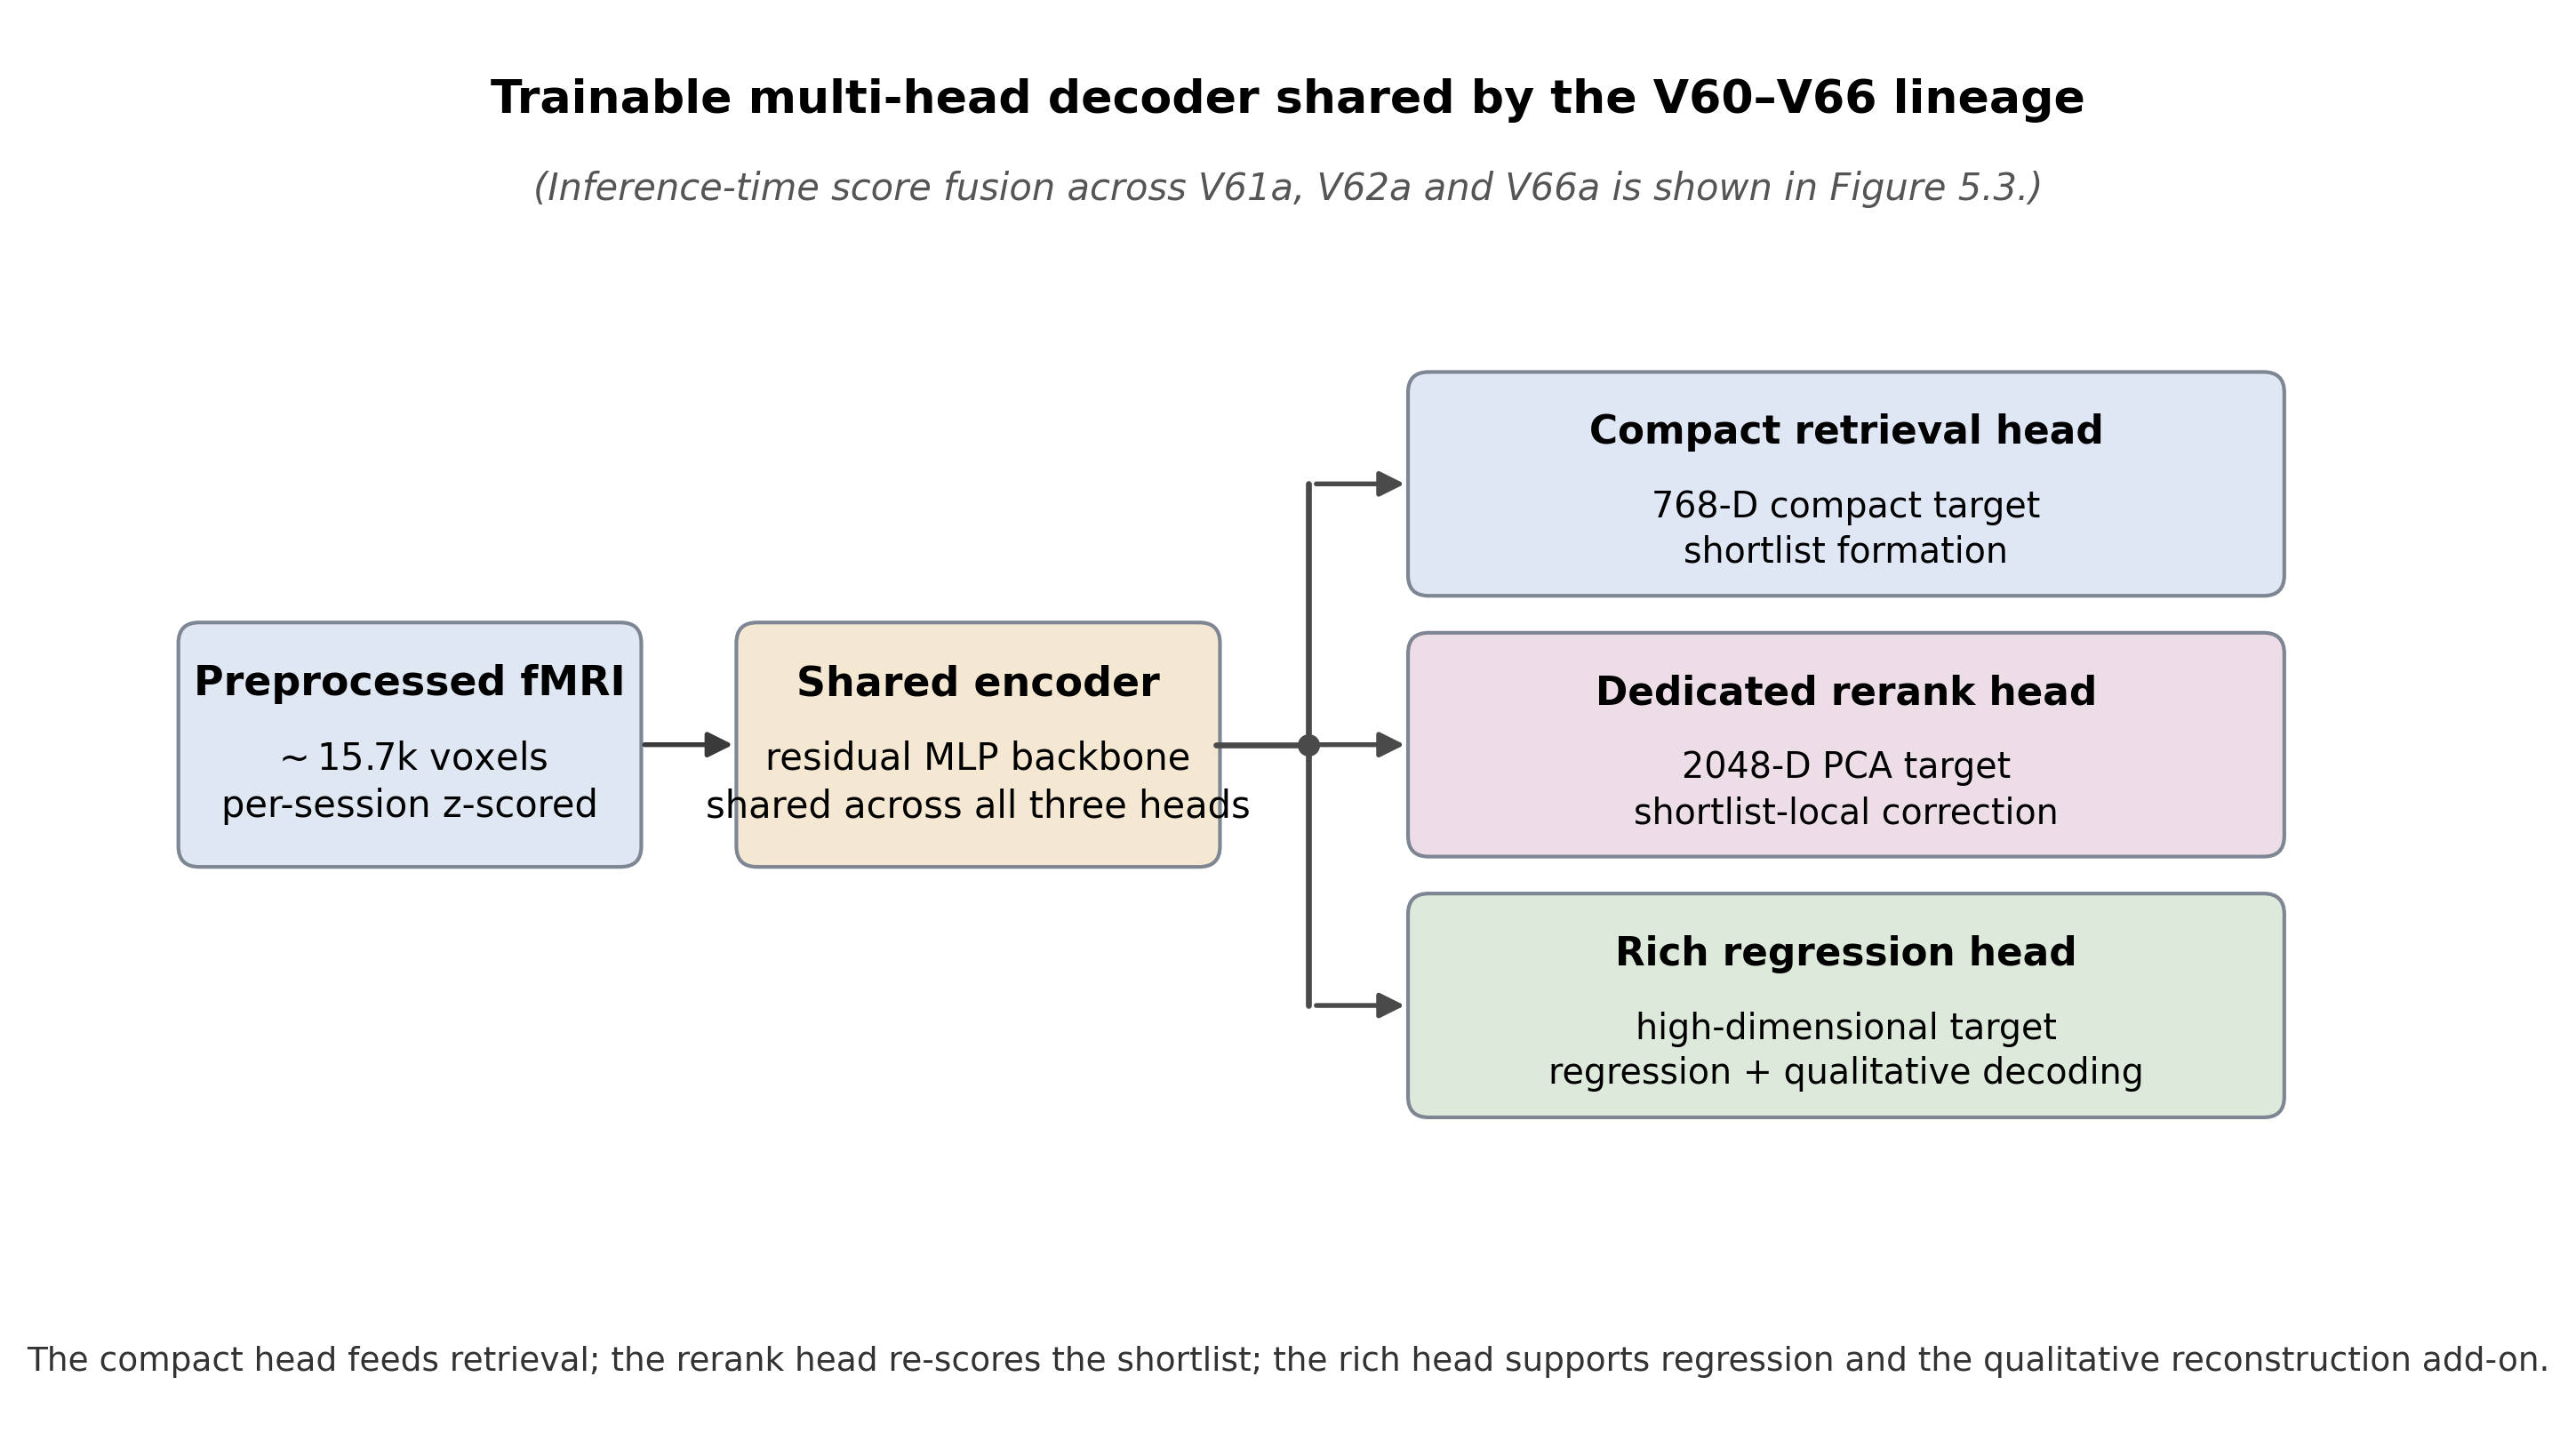
\includegraphics[width=\textwidth]{model_architecture.png}
    \caption{Trainable multi-head decoder shared by the V60--V66 lineage. A residual MLP encoder operates on the preprocessed voxel vector and feeds three task-specific heads (compact for shortlist, rerank for shortlist-local correction, rich for regression-style targets and qualitative decoding). This is the trainable architecture; the inference-time score fusion across V61a, V62a, and V66a that yields the headline SHARED1000 result is described in Section~\ref{chap:experiments} and depicted separately in Figure~\ref{fig:triple_fusion_architecture}.}
    \label{fig:model_architecture}
\end{figure}

\section{Inference and Score Fusion}

At inference time, the compact head first retrieves a shortlist of candidate images. Let $\mathcal{S}_K(x_i)$ denote the top-$K$ shortlist obtained from compact retrieval. In the earlier V30/V32 wave, the rerank head rescales those candidates locally. If $s_c(i,j)$ is the compact score and $s_r(i,j)$ is the rerank score for candidate $j$ in the shortlist of sample $i$, the shortlist-local fused score can be written as
\begin{equation}
s_{\mathrm{fusion}}(i,j) = \alpha \, s_c(i,j) + (1-\alpha) \, s_r(i,j), \qquad j \in \mathcal{S}_K(x_i),
\label{eq:fusion_score}
\end{equation}
where $\alpha \in [0,1]$ is a fusion weight. This formulation established the key methodological lesson of the thesis: reranking is most effective as a corrective signal applied inside a strong shortlist.

A first frozen fixed-fusion system extends this idea with a complementary legacy expert. Using z-score-normalized expert scores, the corresponding score combination can be written as
\begin{equation}
s_{\mathrm{milestone}}(i,j) = 0.3\,\widetilde{s}_{c,\mathrm{CSLS}}(i,j) + 0.7\,\widetilde{s}_{\ell,\mathrm{CSLS}}(i,j),
\label{eq:best_fusion_score}
\end{equation}
with $\widetilde{s}_{c,\mathrm{CSLS}}$ denoting the normalized compact-CSLS score from V35 and $\widetilde{s}_{\ell,\mathrm{CSLS}}$ denoting the normalized legacy-CSLS score from N1v28a. The rerank branch remains methodologically important and still informs the architecture; the V35 plus legacy combination is retained as a milestone result that validates the compact--rerank--rich decomposition under expert fusion.

After validating this compact, rerank, and rich decomposition, the final inference-time extension explored stronger token-space decoding and cross-architecture score fusion. The exported best system replaces the two-expert fusion above with a frozen score-level combination of three retrieval experts that span different target spaces and different inductive biases: a 197K token-space model (V61a) evaluated with 16-draw Monte Carlo test-time augmentation (MC-TTA-16), a 768-D CLS retrieval model (V62a), and a 768-D ROI-pretrained model (V66a). With $\widetilde{s}_{1,\mathrm{CSLS}}$, $\widetilde{s}_{2,\mathrm{CSLS}}$, and $\widetilde{s}_{3,\mathrm{CSLS}}$ denoting the normalized CSLS scores of these three experts, the final retrieval score is
\begin{equation}
s_{\mathrm{final}}(i,j) = 0.7\,\widetilde{s}_{1,\mathrm{CSLS}}(i,j) + 0.1\,\widetilde{s}_{2,\mathrm{CSLS}}(i,j) + 0.2\,\widetilde{s}_{3,\mathrm{CSLS}}(i,j),
\label{eq:triple_fusion_score}
\end{equation}
evaluated with CSLS neighbourhood size $k=3$. The weights, the CSLS neighbourhood size, and the choice of experts are all frozen before SHARED1000 evaluation, so the final system performs no test-time tuning. The final fusion is applied only at the retrieval-score level: it combines normalised CSLS score matrices from \emph{independently trained} retrieval experts and does not define a single fused latent representation. Equation~\eqref{eq:triple_fusion_score} is therefore not an end-to-end jointly trained fusion architecture and shares no decoder weights between the three experts; the trainable multi-head decomposition described in Section~\ref{sec:architecture_evolution} and depicted in Figure~\ref{fig:model_architecture} characterises the V30/V35 family, while V61a, V62a, and V66a are separate fine-tuned models whose only point of interaction is Equation~\eqref{eq:triple_fusion_score}.

A useful way to interpret the overall design is therefore that the first stage solves a difficult global search problem, the rerank branch provides shortlist-local discrimination, the two-expert milestone fusion validates that complementary experts can be combined at inference time, and the final triple fusion combines partially different information from three target spaces and architecture families through frozen score-level weights, without retraining the backbone. This division of labour is one of the main methodological lessons of the project.

\section{Reproducibility Principles}

A significant part of the methodology is dedicated to reproducibility. The project maintains versioned experiment configurations, cached targets, explicit split logic, and a strict separation between training-time and evaluation-time computations. This is especially important in a thesis context because the scientific value of the results depends not only on the final metric values, but also on the ability to explain why those values were obtained and how they changed across experimental waves.

The practical implication is that every experiment is treated as a traceable artifact with explicit inputs, outputs, and evaluation scripts. In a research area where silent alignment bugs can invalidate an otherwise sophisticated system, reproducibility is not just a software-engineering virtue; it is a core scientific requirement.


\chapter{Software Design, Implementation, and Validation}
\label{chap:implementation}

\section{Analysis and Design Goals}

Because the thesis contains an implemented software system, the written document should reflect the essential stages of the application life cycle: analysis, design, implementation, and testing. In this project, the analysis stage identified four non-negotiable requirements. First, the system had to preserve strict alignment between each fMRI sample and its visual target. Second, it had to support rapid experimental iteration without silently changing the evaluation protocol. Third, it had to make it easy to compare model versions under a common metric suite. Fourth, it had to remain reproducible enough that every reported result could be traced back to a concrete configuration and checkpoint.

These requirements informed the high-level design of the pipeline. Instead of building a monolithic training script, the system was organized around loosely coupled stages: data preparation, target extraction and caching, model training, evaluation, result aggregation, and qualitative analysis. This decomposition reduces implementation risk and makes scientific debugging more transparent. If an experiment fails, the author can determine whether the failure is caused by preprocessing, target generation, optimization, or evaluation rather than treating the whole project as a black box.

\section{Software Architecture}

At a conceptual level, the implemented system follows a staged architecture:
\begin{enumerate}[leftmargin=1.8em]
    \item \textbf{Data layer:} loading NSD-derived features, image identifiers, subject/session metadata, and split definitions;
    \item \textbf{Target layer:} extracting, caching, and reusing CLIP-based latent targets and derived variants;
    \item \textbf{Model layer:} defining baseline and multi-head decoders together with their losses and optimization logic;
    \item \textbf{Evaluation layer:} computing retrieval metrics, shortlist reranking, fusion scores, and summary tables;
    \item \textbf{Analysis layer:} storing experiment manifests, qualitative outputs, plots, and leaderboard-style comparisons.
\end{enumerate}

This architecture is intentionally research-oriented. Its purpose is not only to train a model, but also to preserve experimental meaning and make repeated ablations comparable.

\begin{figure}[htbp]
    \centering
    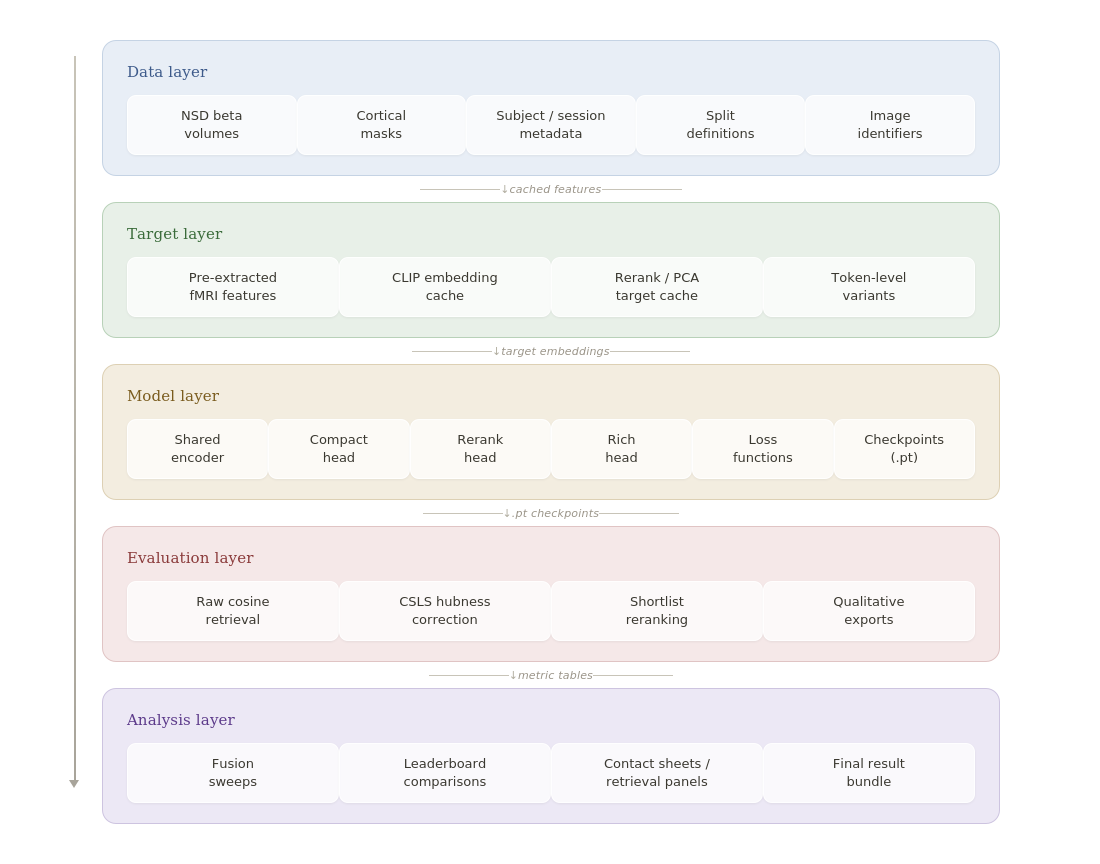
\includegraphics[width=0.92\textwidth]{software_architecture.png}
    \caption{Software architecture of the research pipeline. The implementation is deliberately layered so that data preparation, target caching, training, evaluation, and qualitative export remain traceable and reproducible.}
    \label{fig:software_architecture}
\end{figure}

\section{Configuration Management and Versioning}

A recurring difficulty in research software is that experiments drift over time: hyperparameters change, split definitions evolve, and intermediate artifacts are overwritten. To avoid this, the pipeline is organized around versioned experiment configurations. Each major experiment wave is associated with an explicit configuration file that records data sources, target choices, architecture hyperparameters, loss weights, training settings, and evaluation options.

Versioning is especially important in this thesis because the experimental narrative depends on comparing multiple iterations rather than reporting only a single final run. When a new idea is tested, the goal is not merely to obtain a number but to understand whether a change in the score is caused by the underlying modelling idea or by a hidden change in the protocol. Configuration versioning therefore supports both reproducibility and interpretability.

\section{Implementation of the Training and Evaluation Flow}

The implementation flow can be summarized as follows. First, NSD-derived samples are loaded and normalized under a split-aware preprocessing regime. Second, target latents are either extracted on demand or retrieved from caches, reducing repeated compute and eliminating inconsistencies between experiments. Third, the selected decoder is trained with a loss appropriate to the experiment family. Fourth, validation-time retrieval is computed on a fixed gallery, together with CSLS correction and shortlist reranking when applicable. Finally, results are aggregated into human-readable summaries and compared against previous runs.

A useful abstraction is to think of the whole system as a deterministic map
\begin{equation}
\mathcal{P}:(\mathcal{D},\mathcal{C},\mathcal{A}) \longmapsto \mathcal{R},
\label{eq:pipeline_map}
\end{equation}
where $\mathcal{D}$ denotes the data and split definition, $\mathcal{C}$ the configuration, $\mathcal{A}$ the cached artifacts and checkpoints, and $\mathcal{R}$ the resulting metrics and qualitative outputs. The advantage of this view is that it clarifies what must remain fixed when two experiments are compared.

\section{Validation and Testing Strategy}

In the present project, testing took several complementary forms:
\begin{itemize}
    \item \textbf{split-integrity checks}, ensuring that repeated images or derived artifacts cannot leak across train and validation sets;
    \item \textbf{shape and alignment checks}, verifying that every prediction matrix corresponds exactly to its intended ground-truth target matrix;
    \item \textbf{metric sanity checks}, confirming that retrieval metrics behave as expected on controlled inputs;
    \item \textbf{checkpoint and cache verification}, ensuring that the correct artifacts are loaded during evaluation;
    \item \textbf{qualitative inspection}, used to detect failure modes that aggregate metrics can hide.
\end{itemize}

This testing strategy is substantial enough to be regarded as part of the thesis contribution. Several improvements in the final system did not come from inventing a new loss function, but from identifying and eliminating hidden sources of inconsistency. In that sense, rigorous validation acted as a performance multiplier.

\begin{figure}[htbp]
    \centering
    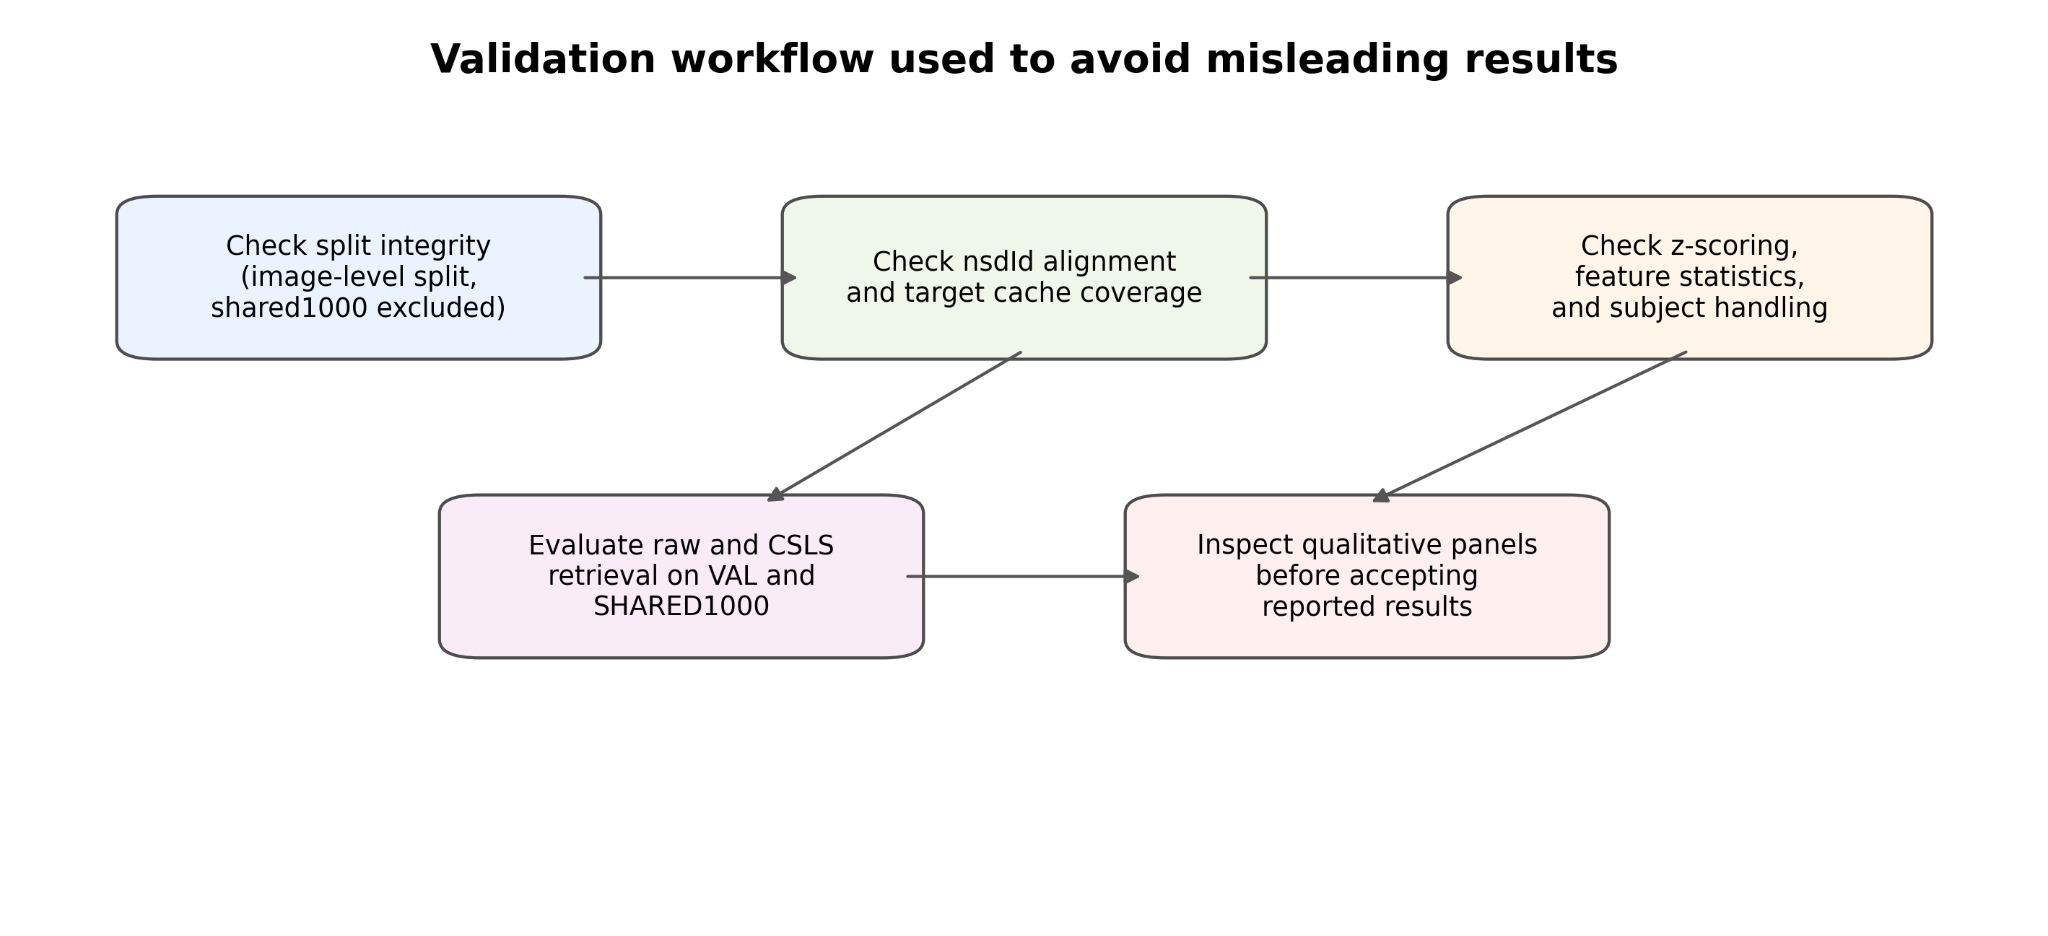
\includegraphics[width=0.95\textwidth]{validation_workflow.png}
    \caption{Validation workflow used throughout the thesis. Raw metric values are only trusted after split integrity, alignment, normalization, and qualitative inspection have been verified.}
    \label{fig:validation_workflow}
\end{figure}

\section{Reproducibility, Artifact Management, and Reporting}

Reproducibility in this thesis is supported by explicit artifact management. Targets, checkpoints, predictions, and summary outputs are stored as named and versioned artifacts. This makes it possible to revisit a result months later and still recover its provenance. Such traceability is essential in a long-running experimental project, especially when results evolve across many versions.

The reporting layer is equally important. Tables, plots, retrieval examples, and diagnostic summaries are not treated as cosmetic additions but as part of the scientific record. For example, a metric table may reveal that rerank-only retrieval underperforms globally, while a shortlist-local diagnostic may show that the rerank head still contains useful discriminative information. Only by keeping both artifact provenance and reporting structure under control can such nuanced conclusions be justified.



\chapter{Experiments, Results, and Discussion}
\label{chap:experiments}

\paragraph{Note on experiment identifiers.}\label{par:experiment_id_note}
Throughout this chapter, identifiers such as V30, V35, V61a, V62a, V66a, and N1v28a denote repository-traceable experiment instances: each identifier refers to a concrete configuration file, checkpoint, and exported metrics artifact (Table~\ref{tab:artifact_map}). They are shorthand for implementation instances, not names of standalone methods in the literature sense. Accordingly, the scientific comparisons below are always between the associated design choices---for example target space, decoder structure, reranking strategy, or score-fusion recipe---rather than between the identifiers themselves. Where helpful, the three retrieval experts are also referred to descriptively as the \emph{token-space expert} (V61a), the \emph{CLS expert} (V62a), and the \emph{ROI-pretrained expert} (V66a).

\section{Experimental Strategy}

The experimental strategy of the thesis is iterative. Instead of moving directly to the most complex architecture, the project first established strong baselines, then diagnosed failure modes, and only afterward introduced richer representation choices, multi-head decoders, and expert fusion. This approach is important because, in brain decoding, implementation errors and evaluation mismatches can easily masquerade as modelling limitations.

The history of the project reveals four broad phases. The first phase stabilizes the pipeline by validating sample--target alignment, correcting training pathologies, and confirming that evaluation measures true image-specific retrieval under a leakage-free protocol. The second phase investigates richer target spaces and multi-head retrieval design, culminating in the V30/V32 family where compact retrieval, reranking, and rich regression are explicitly separated. The third phase introduces expert complementarity: a stronger V35 base is combined at inference time with an earlier complementary baseline expert, providing the V35 plus N1v28a fixed-fusion milestone. The fourth phase extends this idea to a cross-architecture, cross-target-space score fusion that uses a 197K token-space model with MC-TTA and two complementary 768-D experts, yielding the final exported retrieval system reported in the thesis.

\begin{figure}[htbp]
    \centering
    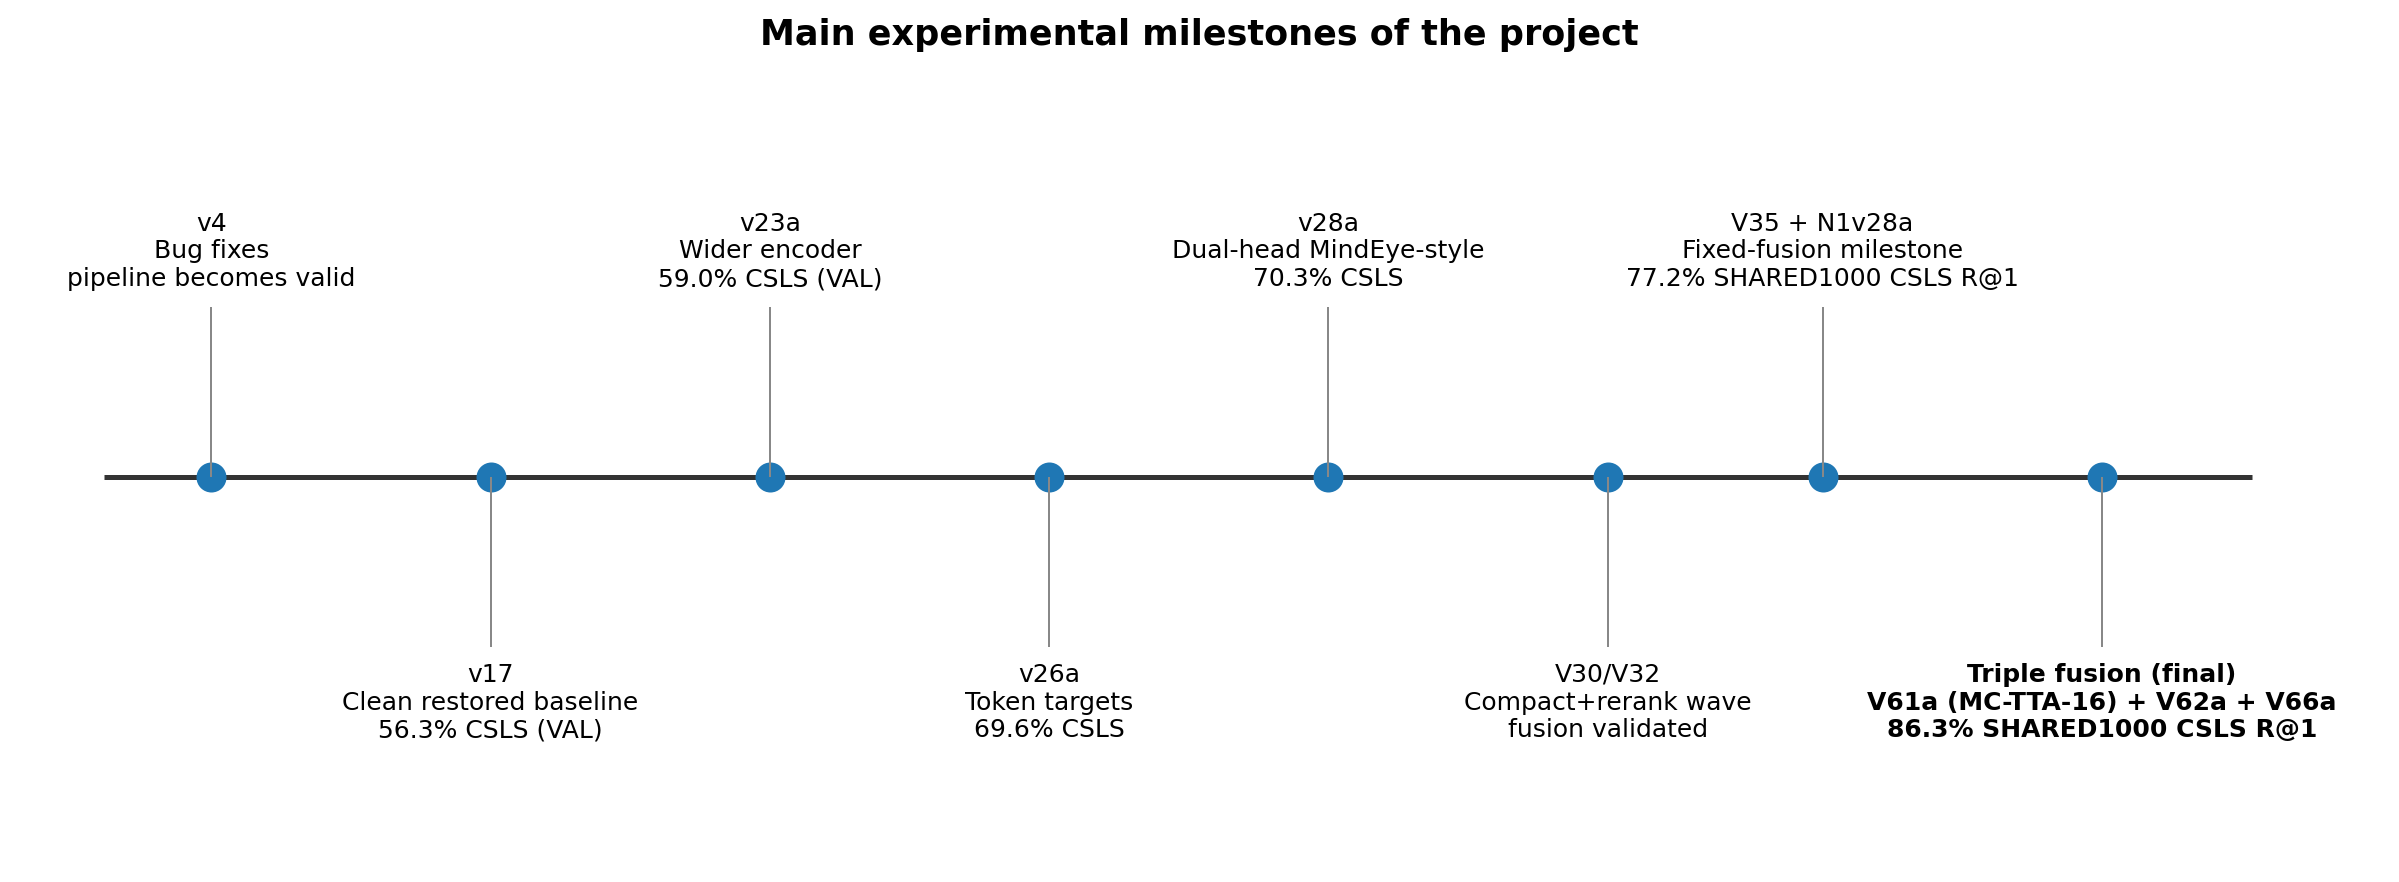
\includegraphics[width=\textwidth]{experiment_timeline.png}
    \caption{Main milestones of the experimental trajectory. The horizontal axis is not a metric scale; the figure highlights the turning points that shaped the project, ending with the cross-architecture triple-fusion exported system.}
    \label{fig:experiment_timeline}
\end{figure}

\section{Evaluation Protocol}

All experimental comparisons in the thesis are interpreted under a fixed retrieval-oriented evaluation protocol. The main endpoints are validation Recall@1 and SHARED1000 Recall@1, with CSLS-corrected retrieval used whenever hubness is relevant. This choice reflects the actual scientific question of the thesis: whether the predicted latent representation is discriminative enough to recover the correct stimulus image from a gallery.

The evaluation protocol is deliberately conservative. The validation split is used for model selection, fusion selection, and qualitative inspection; SHARED1000 is treated as the external benchmark split. When multiple experts are combined, the chosen recipe is selected on validation and then frozen before being applied to SHARED1000. This means that the final best system does not rely on test-time tuning.

\begin{table}[htbp]
\centering
\small
\begin{tabularx}{\textwidth}{>{\raggedright\arraybackslash}p{4.0cm} >{\raggedright\arraybackslash}X}
\toprule
\textbf{Setting} & \textbf{Value} \\
\midrule
Subject & subj01 (NSD subject 01); the V60--V66 experiment family configs target this single-subject setting verbatim \\
Dataset & Natural Scenes Dataset (NSD) \cite{Allen2022} \\
Region of interest & \texttt{nsdgeneral} cortical mask \\
Stimulus split & image-level (no stimulus appears in more than one of train / validation / SHARED1000) \\
Train / validation ratio & $90\%$ / $10\%$ at image level, with \texttt{split\_by\_image=True} in the experiment configs \\
SHARED1000 benchmark & $1000$ stimuli held out from training and validation; used only after the fusion recipe is frozen \\
Repeated trials & not averaged at training time; \texttt{average\_repetitions=false} preserves single-trial fMRI \\
Normalisation & per-session $z$-score on the fMRI feature vector, with statistics estimated on train trials only \\
Leakage prevention & each unique stimulus image is assigned to exactly one of train / validation / SHARED1000; \texttt{exclude\_shared1000=true} during training \\
\bottomrule
\end{tabularx}
\caption{Data, split, and protocol summary for the V60--V66 retrieval experiment family. Values reproduced verbatim from the YAML configs of V61a, V62a, and V66a in \texttt{configs/experiments/}.}
\label{tab:protocol}
\end{table}

\section{Qualitative Interpretation of the Experimental Evolution}

A major lesson of the project is that progress came more from disciplined diagnosis of bottlenecks than from arbitrary increases in architectural complexity, and from separating the decoding problem into the distinct roles of compact retrieval, shortlist-local reranking, and rich latent regression rather than forcing a single representation to satisfy all of them. Table~\ref{tab:experimental_waves} summarises the resulting experiment families: early debugging established a leakage-free pipeline; latent-space enrichment showed that richer targets help but also create harder retrieval geometry; multi-head retrieval validated the separation of roles; and inference-time expert fusion---first as a two-expert milestone, then as the final cross-architecture triple-fusion system---then exploits complementary experts without retraining the backbone.

\begin{table}[htbp]
\centering
\small
\begin{tabularx}{\textwidth}{>{\raggedright\arraybackslash}p{2.7cm} >{\raggedright\arraybackslash}p{3.4cm} >{\raggedright\arraybackslash}X}
\toprule
\textbf{Experiment family} & \textbf{Main question} & \textbf{Main lesson} \\
\midrule
Baseline stabilization & Is the pipeline aligned and leakage-free? & Trustworthy experiments require correct sample/target alignment before any architecture scaling \\
Latent-space enrichment & Do richer or more structured targets help? & Target quality matters, but richer spaces also create harder retrieval geometry and stronger hubness effects \\
Multi-head retrieval design & Should one model solve all retrieval roles at once? & Separating compact retrieval, reranking, and rich regression is more effective than forcing one universal latent space \\
Compact--rerank fusion & Can reranking act as a corrective signal? & Yes; shortlist-local fusion improves over compact retrieval alone and validates the multi-stage design \\
Frozen expert fusion & Can complementary experts improve the exported system without retraining the whole backbone? & Yes; the V35 compact expert combined with the earlier complementary baseline expert N1v28a under fixed normalized-weighted fusion establishes a strong milestone \\
Cross-architecture triple fusion & Can experts from different target spaces and different architectures be combined at inference time? & Yes; a frozen triple score fusion across a 197K token-space model with MC-TTA and two complementary 768-D experts becomes the final exported system \\
\bottomrule
\end{tabularx}
\caption{High-level summary of the major experiment families in the thesis.}
\label{tab:experimental_waves}
\end{table}

\section{Final Retrieval Results}

The final exported system is a frozen score-level combination of three independently trained retrieval experts spanning different target spaces and inductive biases: the \emph{token-space expert} (V61a), evaluated with 16-draw Monte Carlo test-time augmentation; the \emph{CLS expert} (V62a) operating in a 768-D ViT-L/14 CLS target space; and the \emph{ROI-pretrained expert} (V66a) in a 768-D ROI-pretrained target space. Their CSLS-corrected score matrices are $z$-score normalised and combined under fixed weights $w_1/w_2/w_3 = 0.7/0.1/0.2$ with CSLS neighbourhood size $k=3$, all chosen on validation and frozen before SHARED1000, so the primary retrieval result does not depend on test-time tuning. The three experts are combined only at score level: they share no decoder weights and the fusion does not define a jointly trained model or a unified fused latent embedding.

Table~\ref{tab:final_results} separates four design stages that should not be conflated: the V30 compact--rerank design stage; the V35 plus N1v28a fixed-fusion milestone; the stronger single-model token-space extension with MC-TTA; and the final frozen cross-architecture triple fusion. SHARED1000 CSLS Recall@1 is treated as the primary held-out benchmark endpoint, because shared-image overlap between pretraining and validation splits in the V60--V66 experiment family can inflate validation metrics relative to the strictly held-out benchmark. Raw percentage points across the 197k-token-space and 768-D CLS targets are reported in the same metric family, but they are not protocol-for-protocol comparable: the two spaces differ in difficulty and hubness geometry, and CSLS only partially mitigates that mismatch.

\begin{table}[htbp]
\centering
\footnotesize
\begin{tabularx}{\textwidth}{>{\raggedright\arraybackslash}p{4.0cm} >{\centering\arraybackslash}p{1.6cm} >{\centering\arraybackslash}p{1.6cm} >{\raggedright\arraybackslash}X}
\toprule
\textbf{System} & \textbf{Raw R@1} & \textbf{CSLS R@1} & \textbf{Interpretation} \\
\midrule
V30e compact head & --- & 49.2\% & First strong compact shortlist head in the V30 design stage \\
V30e compact + rerank fusion & --- & 51.5\% & Validates rerank information inside a strong shortlist \\
V35 + N1v28a fixed fusion & --- & 77.2\% & Previous best; milestone for two-expert fixed fusion \\
V61a (single 197K) & 66.0\% & 79.1\% & Strongest single non-TTA model \\
V64a (continued V61a) & 70.6\% & 78.6\% & Slightly below V61a despite continued training \\
V61a + MC-TTA-16 & 67.3\% & 83.1\% & Strongest single-model variant \\
V62a (768-D CLS) & 39.9\% & 47.5\% & Weak alone; auxiliary expert in the frozen fusion \\
V66a (768-D ROI pretrain) & 35.5\% & 39.1\% & Weak alone; auxiliary expert in the frozen fusion \\
\textbf{Triple fusion V61a$_{\mathrm{mctta16}}$ + V62a + V66a} & \textbf{72.1\%} & \textbf{86.3\%} & \textbf{Final exported system; R@5 = 98.0\%, MRR = 0.914, median rank 1} \\
\bottomrule
\end{tabularx}
\caption{Final retrieval results on SHARED1000, reported as Recall@1 with and without CSLS hubness correction. The V30/V32 compact--rerank design stage and the V35 plus N1v28a fixed fusion are retained as methodological milestones, while the final exported system is the frozen cross-architecture triple score fusion with weights $0.7/0.1/0.2$ and CSLS neighbourhood size $k=3$. SHARED1000 CSLS Recall@1 is treated as the primary SHARED1000 benchmark endpoint.}
\label{tab:final_results}
\end{table}

Relative to the previous V35 plus N1v28a milestone the improvement on SHARED1000 is $+9.1$ percentage points; relative to the token-space expert as a single non-TTA model it is $+7.2$ percentage points; and relative to the token-space expert with MC-TTA-16 it is $+3.2$ percentage points. These gaps are consistent with the three experts contributing partially different information across target spaces and architecture families, which the frozen score-level fusion exploits without retraining the backbone.

\subsection*{Reliability of the fusion improvement}

The $+3.2$ percentage-point gain over the strongest single expert is reported as an aggregate point estimate over $1000$ SHARED1000 trials, alongside a $+1.1$ percentage-point gain at $R@5$ and a parallel rise in $\mathrm{MRR}$ from $0.892$ to $0.914$ (Table~\ref{tab:expert_complementarity}). The thesis does not provide bootstrap $95\%$ confidence intervals or a paired correct-vs-wrong transition table between the strongest single expert and the fusion, because the per-trial fused-rank export for the triple fusion was not preserved beyond the four trials illustrated in Figures~\ref{fig:retrieval_successes_1}--\ref{fig:retrieval_successes_2}. The complementarity claim is therefore supported at the aggregate-metric level only. Re-exporting the per-trial fused ranks across the full benchmark together with a full grid of fusion-weight, CSLS-$k$, and MC-TTA-depth ablations is a priority for a publication-oriented extension; the frozen recipe $0.7/0.1/0.2$ with $k=3$ was itself selected by a small validation-side simplex sweep before SHARED1000 evaluation.

\begin{figure}[htbp]
    \centering
    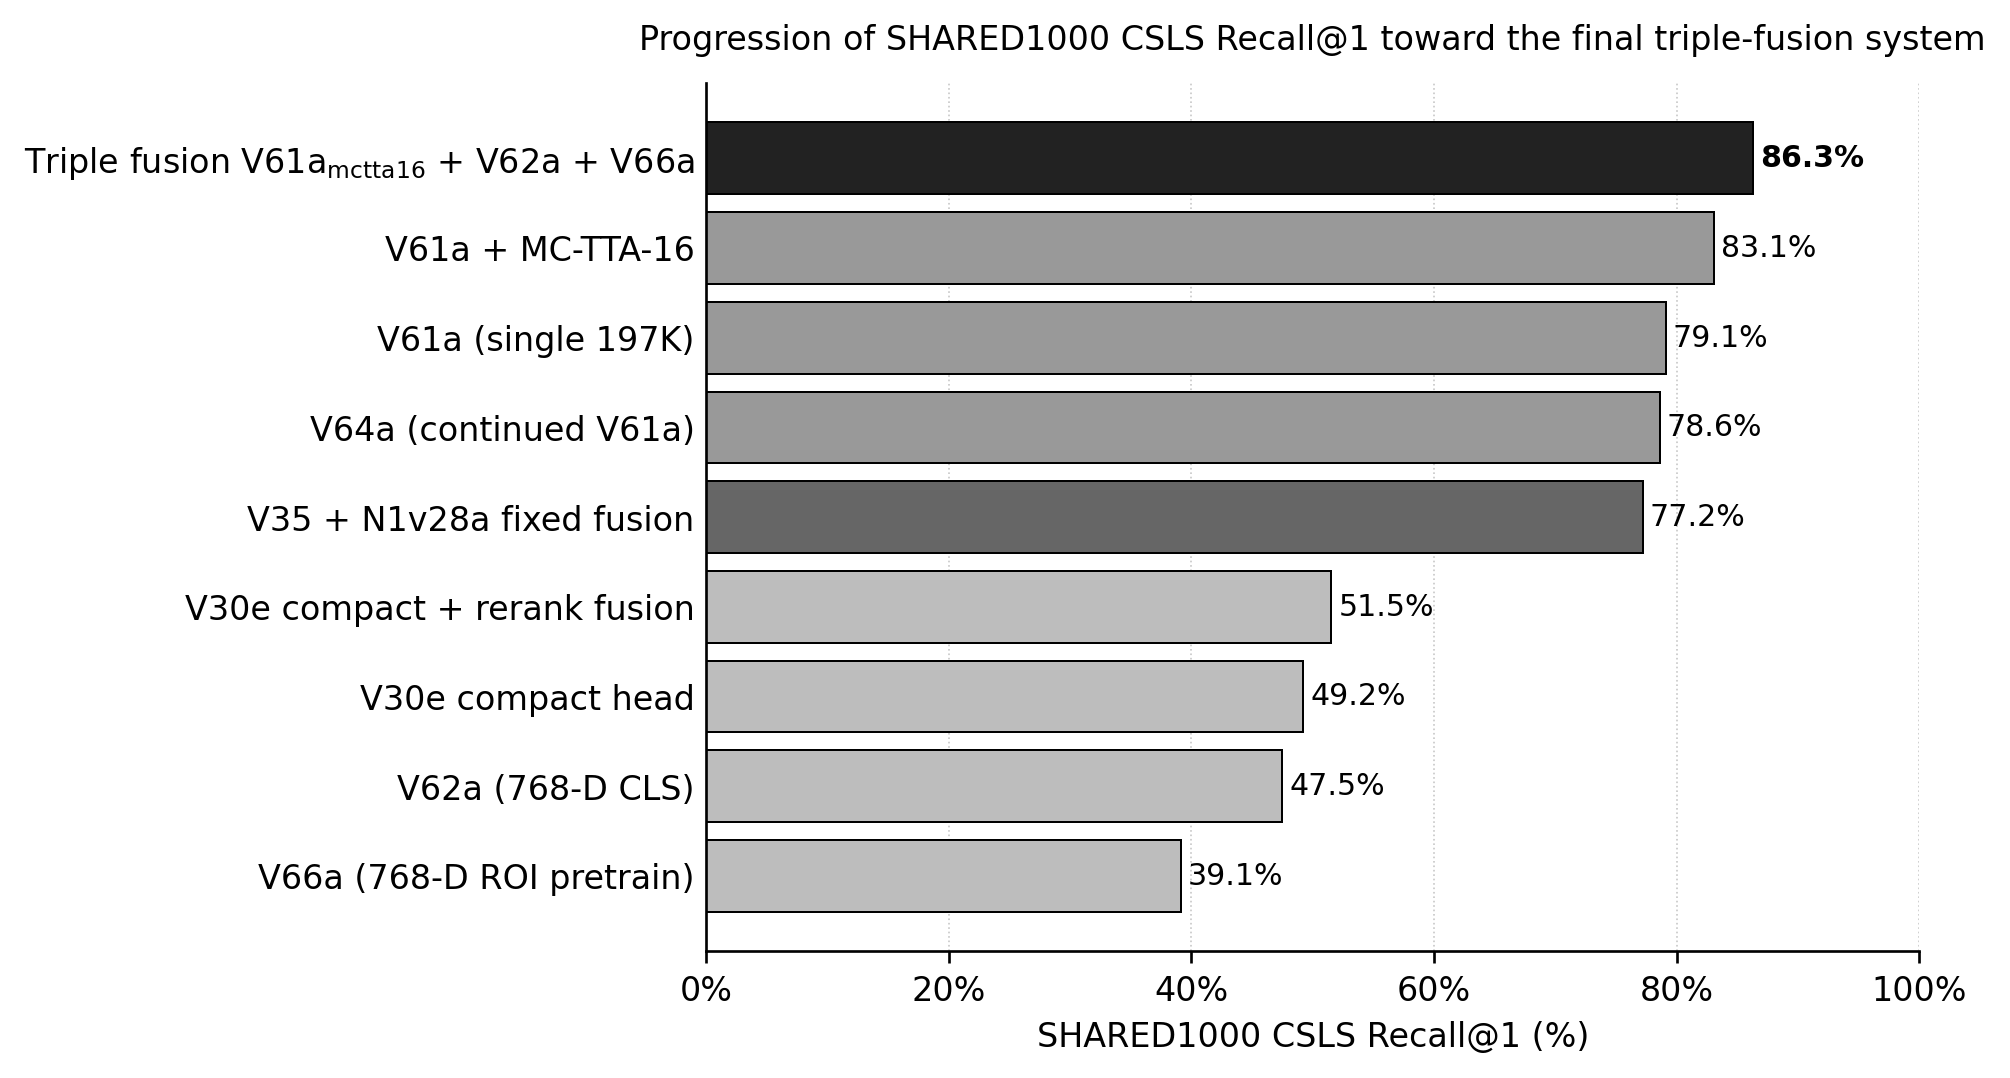
\includegraphics[width=0.90\textwidth]{leaderboard_bar.png}
    \caption{Progression of SHARED1000 CSLS Recall@1 toward the final frozen triple-fusion system. The V35 plus N1v28a fixed fusion is shown as a milestone; the final exported triple fusion of V61a with MC-TTA-16, V62a, and V66a is the highest bar.}
    \label{fig:leaderboard}
\end{figure}

\subsection*{Final cross-architecture fusion extension}

The final extension combines experts that differ along target-space dimensionality and architectural family. The token-space expert (V61a) is the strongest single model in the V60--V66 experiment family; MC-TTA-16 averages $16$ stochastic forward passes with dropout left active at inference and re-normalises the mean on the unit hypersphere, reducing per-trial prediction variance at $16\times$ inference-time compute. The CLS expert (V62a) and the ROI-pretrained expert (V66a) are weaker in isolation but bring geometrically distinct embedding spaces and complementary inductive biases. Their CSLS scores are combined under the fixed weights of Equation~\eqref{eq:triple_fusion_score}; because this is a score-level inference-time fusion, retrieval-geometry claims for the fused system are deferred to the single-expert manifold analyses of Section~\ref{sec:generalization_manifold}. Figure~\ref{fig:triple_fusion_architecture} summarises the three-expert pipeline.

\begin{figure}[t!]
    \centering
    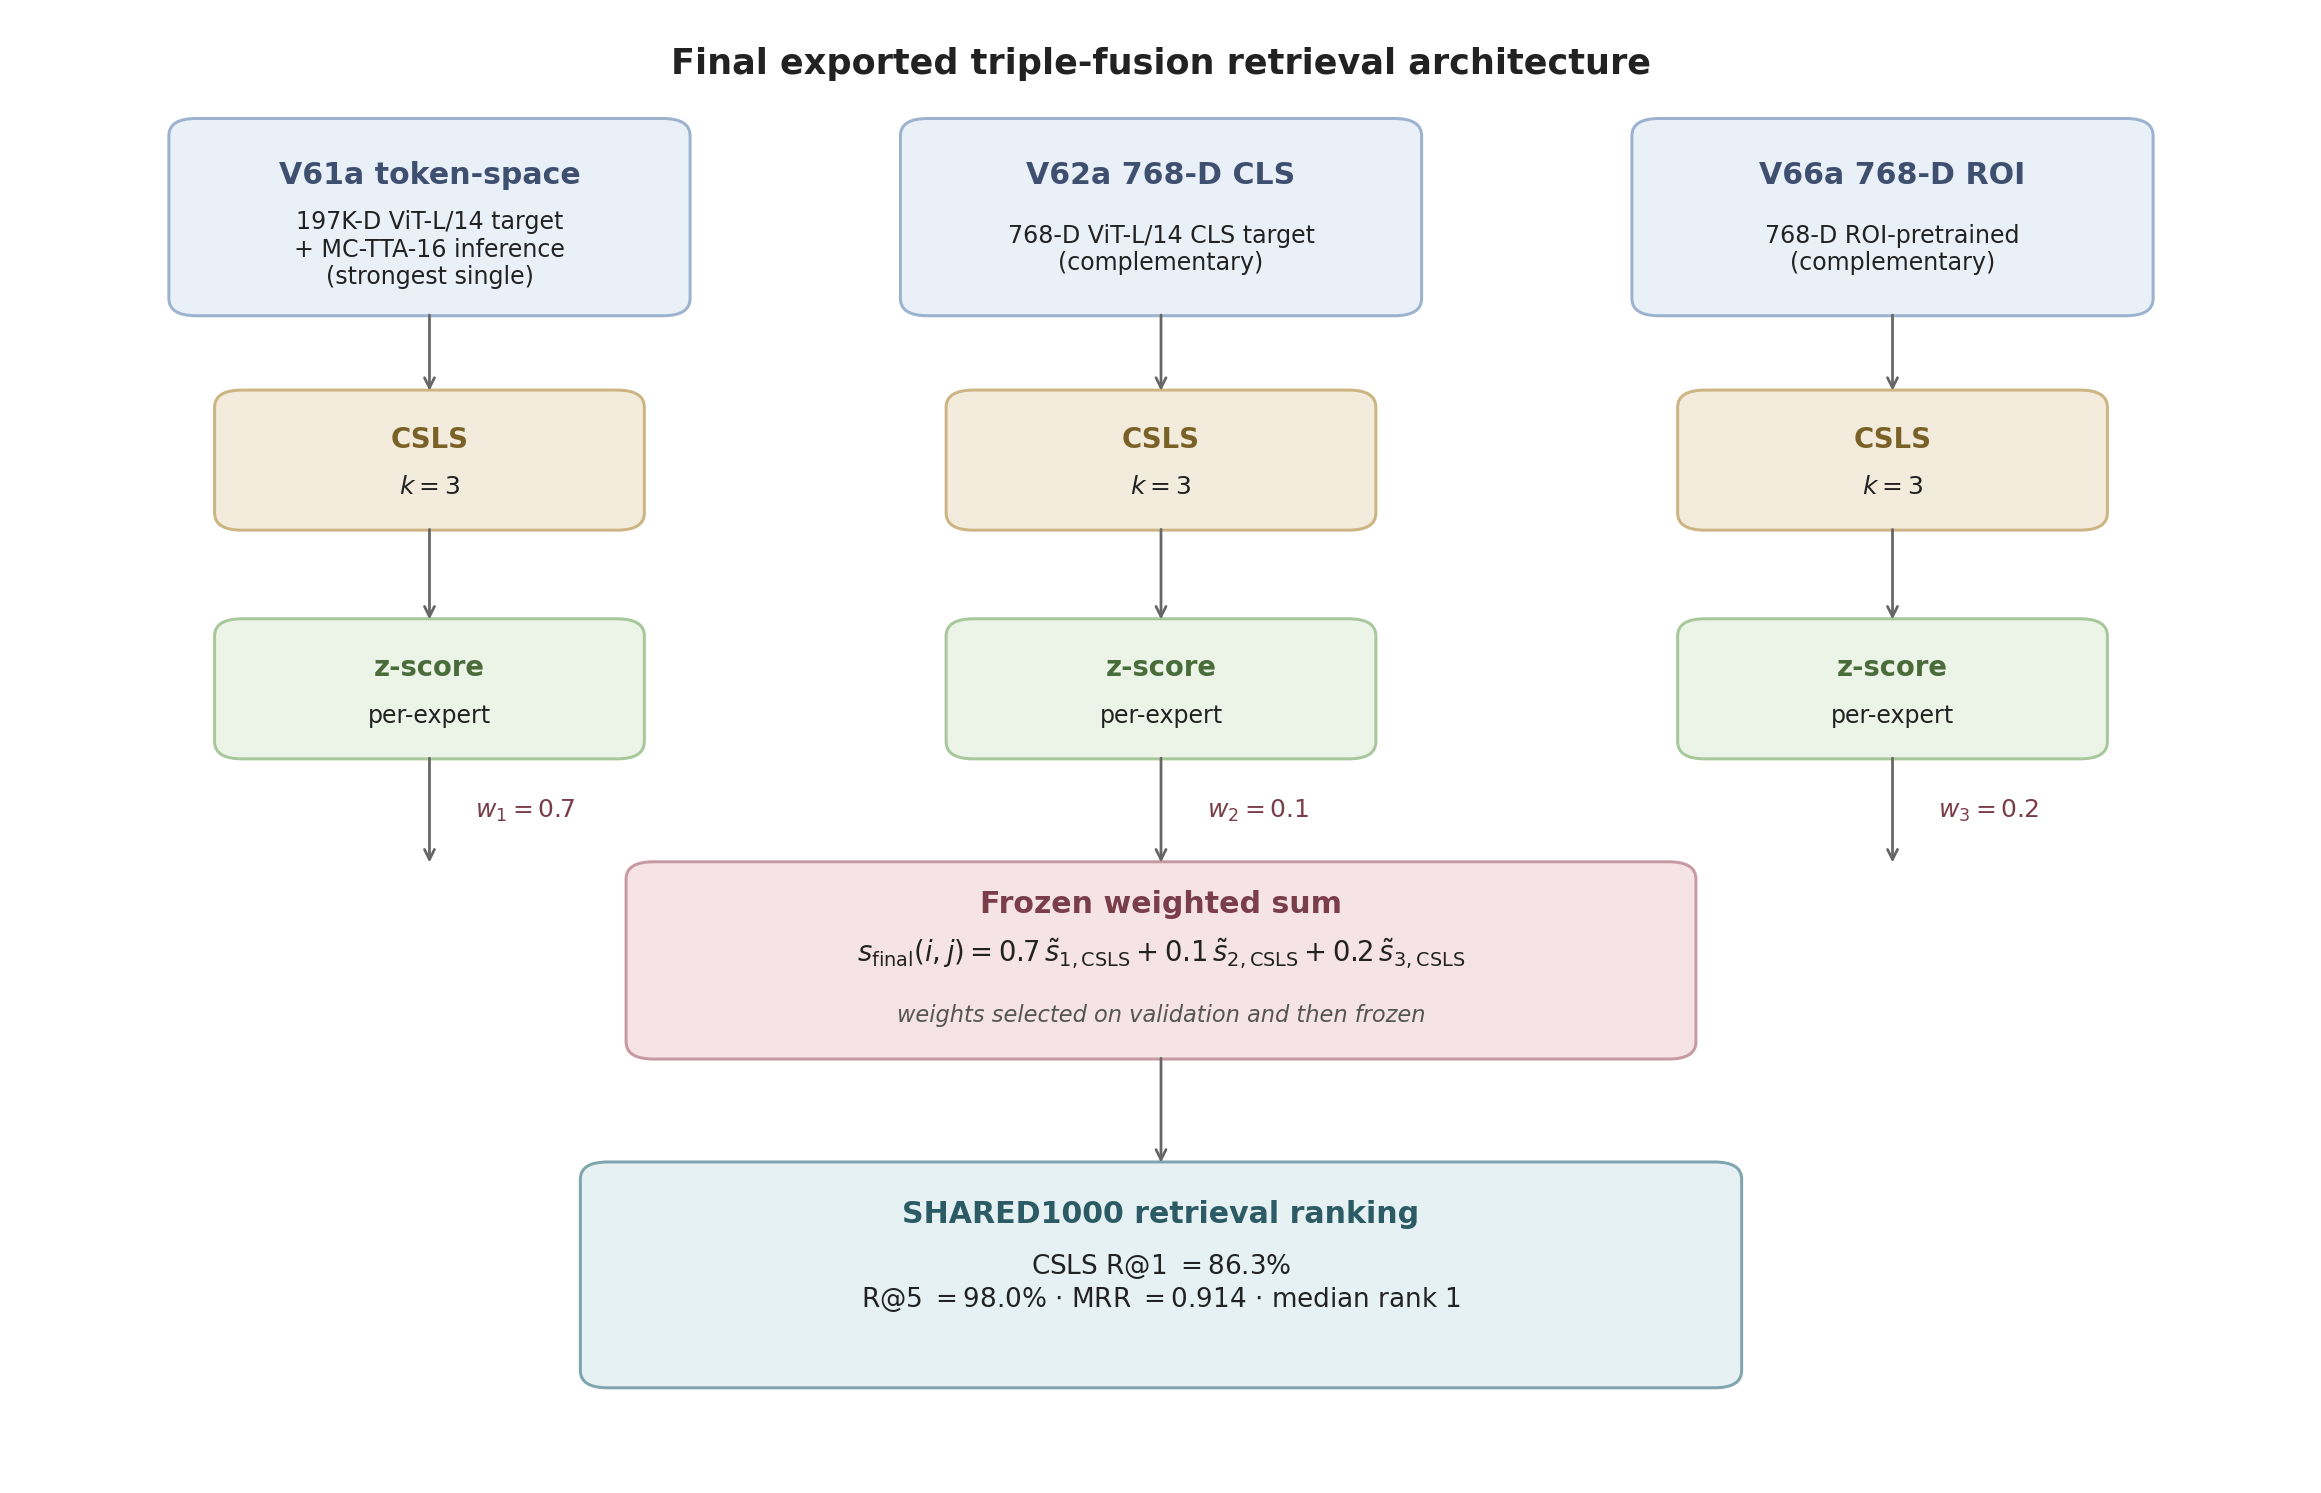
\includegraphics[width=0.95\textwidth]{triple_fusion_architecture.png}
    \caption{Final exported triple-fusion retrieval architecture. The three independently trained experts (V61a token-space with MC-TTA-16, V62a 768-D CLS, V66a 768-D ROI) each produce a CSLS-corrected retrieval score at frozen neighbourhood size $k=3$. The scores are $z$-score normalised per expert and combined by a frozen weighted sum $w_1/w_2/w_3 = 0.7/0.1/0.2$ to produce the SHARED1000 retrieval ranking (CSLS Recall@1 $= 86.3\%$). The combination operates at the retrieval-score level and is applied only at inference time.}
    \label{fig:triple_fusion_architecture}
\end{figure}

\subsection*{Why score-level triple fusion improves retrieval}
\label{sec:why_triple_fusion_anchor}
\label{subsec:why_triple_fusion}

The retrieval gain in Table~\ref{tab:final_results} should not be read as the additive effect of stacking similar experts: the three components of the final system differ in target dimensionality, training objective, and inductive bias, so they fail in measurably different ways at the aggregate level. Table~\ref{tab:expert_complementarity} reports the per-expert SHARED1000 numbers. The 197K token-space expert V61a with MC-TTA-16 dominates each individual ranker, yet the frozen combination still exceeds it on the held-out benchmark even though the two weaker 768-D experts retain non-negligible weights $w_2 = 0.1$ and $w_3 = 0.2$ after validation tuning. That pattern is consistent with complementary correction at the system level. For the bulk of SHARED1000 we do not export per-trial fused ranks in this thesis --- the four illustrated trials in Figures~\ref{fig:retrieval_successes_1} and~\ref{fig:retrieval_successes_2} are the only exception --- and we therefore make no per-trial claim about which specific V61a errors are corrected by V62a or V66a across the full benchmark.

\begin{table}[htbp]
\centering
\footnotesize
\begin{tabularx}{\textwidth}{>{\raggedright\arraybackslash}p{4.0cm} >{\centering\arraybackslash}p{1.4cm} >{\centering\arraybackslash}p{1.4cm} >{\centering\arraybackslash}p{1.4cm} >{\centering\arraybackslash}p{1.4cm} >{\raggedright\arraybackslash}X}
\toprule
\textbf{Expert} & \textbf{CSLS R@1} & \textbf{CSLS R@5} & \textbf{CSLS MRR} & \textbf{Median rank} & \textbf{Role in fusion} \\
\midrule
V61a, 197K token-space, MC-TTA-16 & $83.1\%$ & $96.9\%$ & $0.892$ & $1$ & Dominant ranker ($w_1 = 0.7$) \\
V62a, 768-D CLS & $47.5\%$ & $80.3\%$ & $0.621$ & $2$ & Auxiliary expert with $w_2 = 0.1$ \\
V66a, 768-D ROI-pretrained & $39.1\%$ & $73.8\%$ & $0.545$ & $2$ & Auxiliary expert with $w_3 = 0.2$ \\
\midrule
\textbf{Triple fusion} (frozen) & $\mathbf{86.3\%}$ & $\mathbf{98.0\%}$ & $\mathbf{0.914}$ & $\mathbf{1}$ & Headline exported system \\
\bottomrule
\end{tabularx}
\caption{Per-expert SHARED1000 retrieval metrics under the same 1000-image target-embeddings gallery as the primary benchmark endpoint, and the frozen-weight triple-fusion result they produce. Numbers are reproduced verbatim from the exported fusion summary; the gain over the strongest single expert is $+3.2$ percentage points on CSLS Recall@1 and $+1.1$ percentage points on CSLS Recall@5.}
\label{tab:expert_complementarity}
\end{table}

Three architectural decisions are responsible for converting raw per-expert scores into a usable joint ranking. First, the per-expert CSLS correction at neighbourhood size $k=3$ removes the hubness asymmetries that would otherwise let a small set of generic images dominate retrievals in each space (Section~\ref{sec:generalization_manifold} quantifies this effect for the analyzed expert). Second, the per-expert z-score normalization across the SHARED1000 gallery places all three score streams on a comparable, dimensionless scale before they are summed; raw CSLS scores live in different ranges in the 197K token-space and in the 768-D CLS space, and combining them without normalization would let scale, not information content, decide the result. Third, the weights $w_1/w_2/w_3 = 0.7/0.1/0.2$ are selected on the validation split by sweeping a small simplex, then frozen before the SHARED1000 evaluation; they are not tuned on the held-out benchmark. The weight on V61a reflects its much stronger standalone retrieval, while the smaller weights on V62a and V66a allow auxiliary score streams to influence the final ranking without overwhelming the dominant expert.

The aggregate gain is most visible in the near-miss regime: CSLS Recall@5 rises from $96.9\%$ for the strongest single expert to $98.0\%$ for the fusion, mean reciprocal rank rises in parallel, and the median rank stays at $1$. This signature is more consistent with complementary correction than with redundant ensembling, because redundant experts would mainly reinforce the same top-1 mistakes rather than shorten the tail of slow-decaying ranks. Two caveats apply: the gain holds under a fixed gallery and a fixed weight choice and is not a guarantee about other settings, and because the fusion operates on scalar scores rather than on a unified embedding, the geometric and manifold-level analyses of Section~\ref{sec:generalization_manifold} apply to the V62a single expert, not to the fused system.

\begin{table}[htbp]
\centering
\footnotesize
\begin{tabularx}{\textwidth}{@{}>{\raggedright\arraybackslash}p{2.3cm} >{\raggedright\arraybackslash}X >{\raggedright\arraybackslash}X >{\raggedright\arraybackslash}X@{}}
\toprule
\textbf{Field} & \textbf{V61a (token)} & \textbf{V62a (CLS)} & \textbf{V66a (ROI)} \\
\midrule
Input dim. & \texttt{nsdgeneral} voxels & same & same \\
Target dim. & $197{,}376$ (ViT-L/14 token grid, $257{\times}768$) & $768$ (ViT-L/14 CLS) & $768$ (ViT-L/14 CLS) \\
Encoder & MLP $[8192,8192,4096,2048]$ & MLP $[8192,8192,4096,2048]$ & MLP backbone, $[1024]$ head \\
Decoder head & $[2048]$ projection & $[2048]$ projection & $[1024]$ projection \\
Training losses & vMF-NCE + MSE + $\kappa$ reg.\ + SoftCLIP & vMF-NCE + MSE + $\kappa$ reg.\ + SoftCLIP & vMF-NCE + SoftCLIP + $\kappa$ reg.\ + R-drop \\
Optimiser & AdamW, enc.\ $3\!\cdot\!10^{-6}$, dec.\ $3\!\cdot\!10^{-5}$ & AdamW, enc.\ $3\!\cdot\!10^{-6}$, dec.\ $1\!\cdot\!10^{-5}$ & AdamW, $1\!\cdot\!10^{-4}$ \\
Batch size & $16$ & $64$ & $128$ \\
Epochs & up to $200$, early stop on val.\ R@1 & up to $200$, same criterion & up to $200$, same criterion \\
Inference TTA & MC-dropout, $16$ draws, on-sphere mean (MC-TTA-16) & none & none \\
Fusion weight & dominant, $w_1{=}0.7$ & auxiliary, $w_2{=}0.1$ & auxiliary, $w_3{=}0.2$ \\
\bottomrule
\end{tabularx}
\caption{Final-system implementation summary for the three frozen retrieval experts. All values are reproduced from the YAML configs of V61a, V62a, and V66a in \texttt{configs/experiments/}. The fusion-time hyperparameters are CSLS neighbourhood size $k=3$, per-expert $z$-score normalisation over the SHARED1000 gallery, and frozen weights $w_1/w_2/w_3 = 0.7/0.1/0.2$ (Equation~\eqref{eq:triple_fusion_score}).}
\label{tab:hyperparameters}
\end{table}

\section{Generalization, Robustness, and Manifold Alignment}
\label{sec:generalization_manifold}

The main retrieval gain reported in Table~\ref{tab:final_results} answers a narrow but well-defined generalisation question: given an fMRI response to a held-out stimulus, can the decoder rank the correct image first in a held-out gallery? SHARED1000 is the primary benchmark endpoint because it is held out from training and validation, splits are stimulus-level (so repeated fMRI trials of the same image cannot leak across sets), and the fusion recipe is frozen on validation before being applied. CSLS is used in place of raw cosine because high-dimensional CLIP retrieval suffers from hubness; the analyses below quantify that effect.

\paragraph{Scope of the manifold-alignment analyses.} The geometric analyses summarised in Table~\ref{tab:manifold_evidence} are computed on the V62a single model under the SHARED1000 target-embeddings protocol (1000-image gallery), with the validation split (10000-image gallery) added for context. They therefore characterise the 768-D CLIP-CLS retrieval geometry of one of the three fused experts, not the fused system itself, and are presented as auxiliary evidence that the fMRI-to-CLIP mapping preserves semantic structure rather than as a substitute for the SHARED1000 retrieval endpoint.

\begin{table}[htbp]
\centering
\footnotesize
\begin{tabularx}{\textwidth}{>{\raggedright\arraybackslash}p{3.0cm} >{\raggedright\arraybackslash}p{4.0cm} >{\raggedright\arraybackslash}X >{\raggedright\arraybackslash}p{3.4cm}}
\toprule
\textbf{Evidence type} & \textbf{Metric (source)} & \textbf{What it supports} & \textbf{Caveat} \\
\midrule
Held-out retrieval & Triple-fusion SHARED1000 CSLS R@1 $=86.3\%$ (Table~\ref{tab:final_results}) & Stimulus-level generalization on the primary benchmark endpoint & The primary benchmark endpoint; the only direct claim about the final exported system \\
Hubness control & V62a SHARED1000 hubness Gini cosine $0.386 \rightarrow$ CSLS $0.226$ & CSLS substantially reduces hubness in the analyzed 768-D space & Auxiliary analysis on the V62a expert only \\
Representational geometry & V62a SHARED1000 RSA Spearman $\rho = 0.389$, bootstrap CI $[0.387, 0.392]$ (val.\ $\rho = 0.583$) & Predicted and target RDMs share a stable monotonic structure on the harder benchmark & Single-expert evidence; magnitude drops on the harder split as expected \\
Local neighborhood preservation & V62a SHARED1000 Overlap@10 $= 0.40$ vs random $0.01$, lift $\approx 40\times$ (val.\ lift $\approx 514\times$) & Local CLIP-space neighborhoods are preserved well above chance & Lift depends on gallery size; the SHARED1000 lift is the conservative number \\
Language-space interpretability & V62a SHARED1000 CLIP text-probe agreement@5 $= 0.833$ (29 concepts) and mean semantic-axis Spearman $= 0.673$ across 10 axes & Decoded embeddings agree with CLIP language concepts and preserve interpretable concept directions & Axis quality depends on concept choice; not literal thought decoding \\
\bottomrule
\end{tabularx}
\caption{Generalisation and manifold-alignment evidence. The retrieval row is the primary benchmark endpoint for the fused system; the remaining rows are auxiliary geometric analyses computed on the CLS expert (V62a) under the SHARED1000 protocol (1000-image gallery), with validation values in parentheses.}
\label{tab:manifold_evidence}
\end{table}

\begin{figure}[htbp]
    \centering
    \begin{subfigure}[b]{0.95\textwidth}
        \centering
        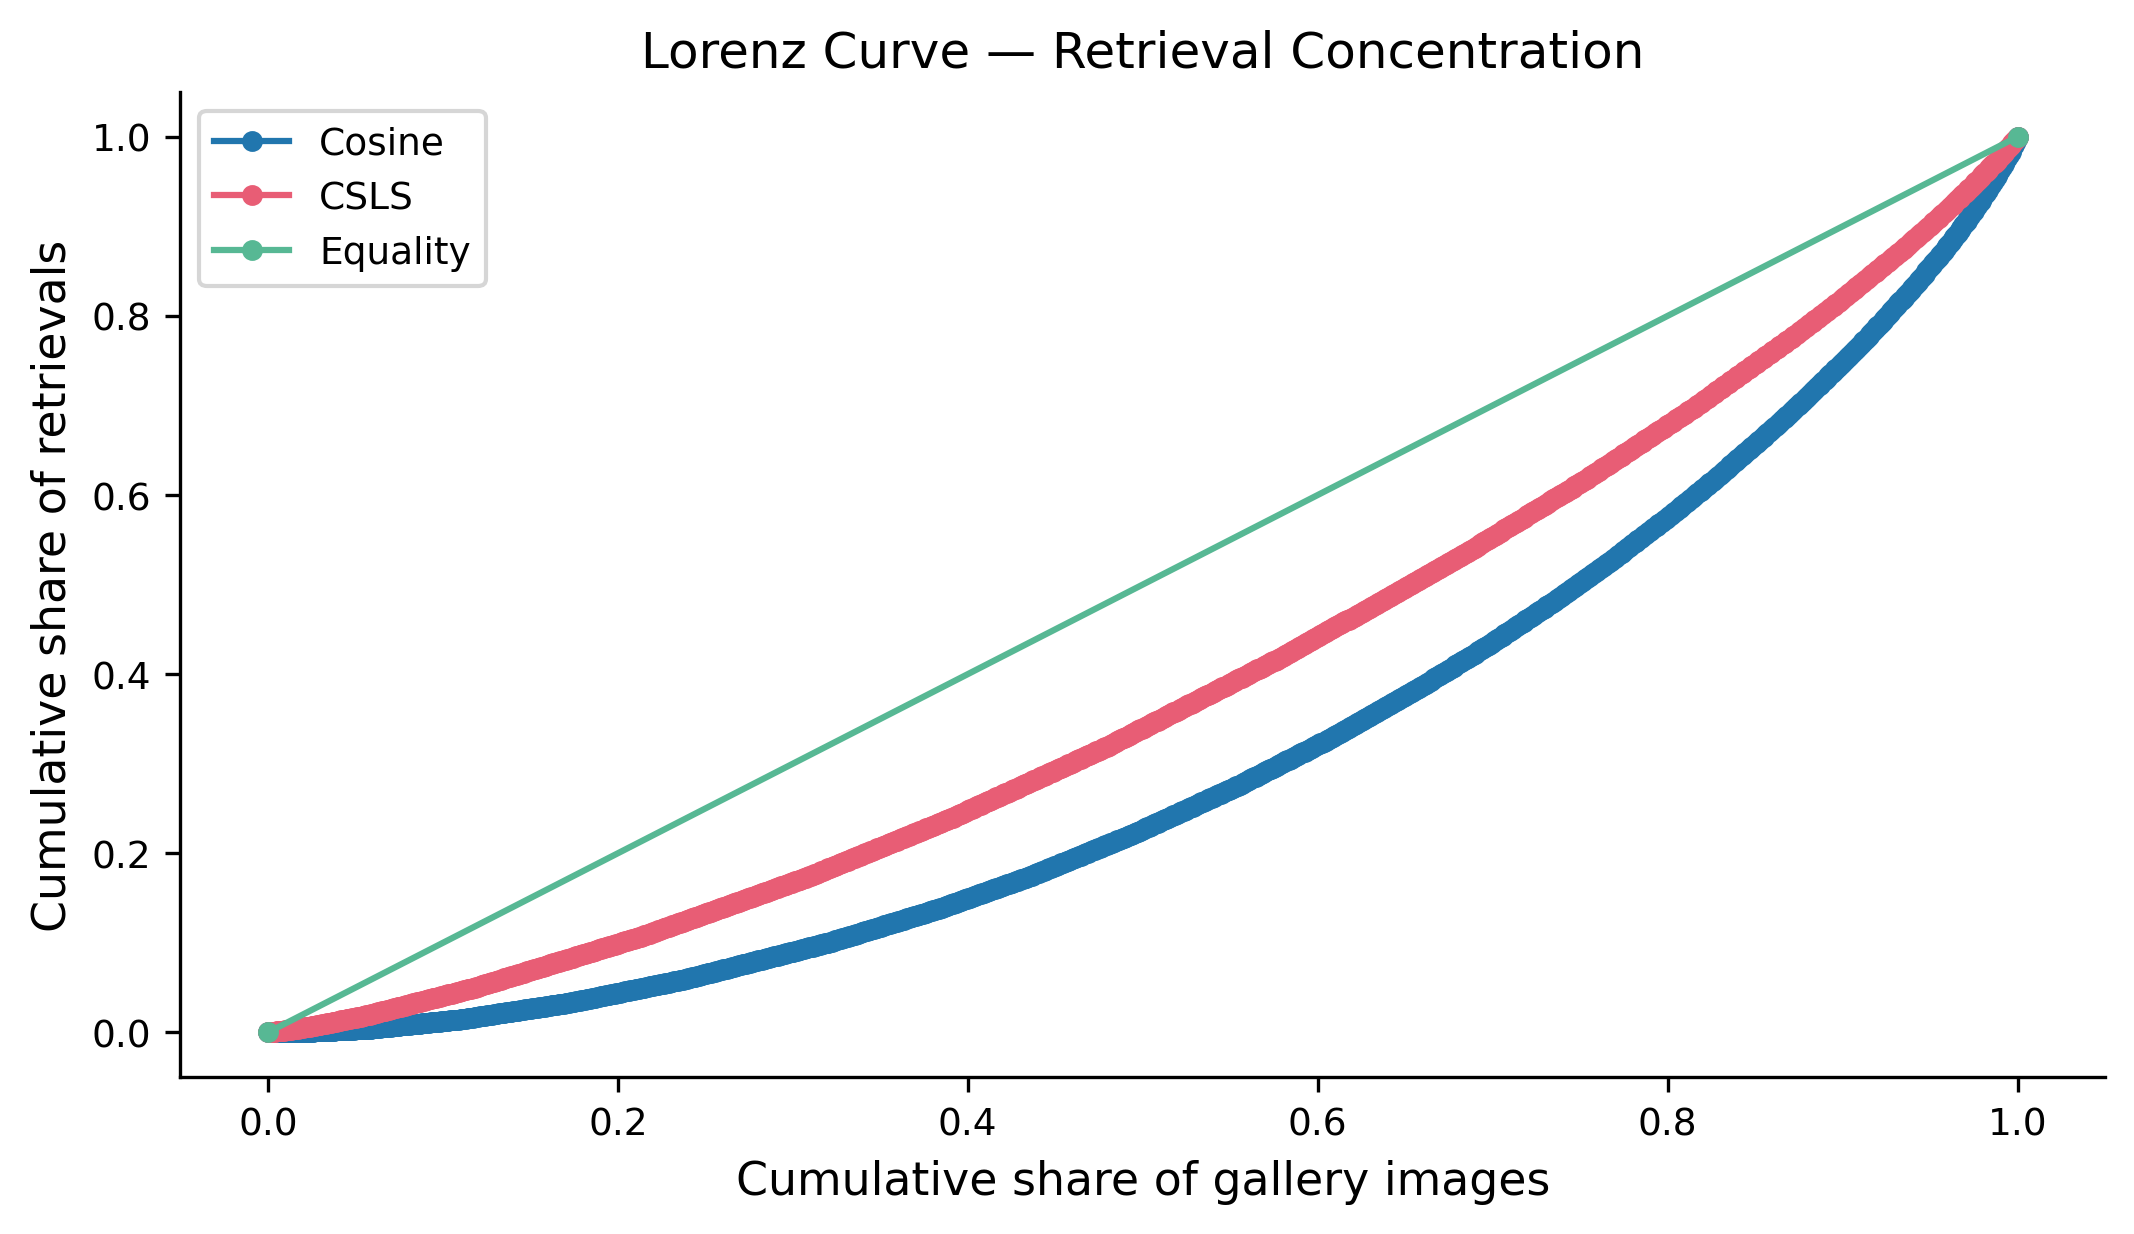
\includegraphics[width=\textwidth]{v62a_hubness_lorenz.png}
        \caption{Hubness Lorenz curves. The CSLS curve is closer to the equality line than the cosine curve, illustrating the reduction of the V62a SHARED1000 hubness Gini from $0.386$ to $0.226$.}
        \label{fig:v62a_lorenz}
    \end{subfigure}

    \vspace{0.6cm}

    \begin{subfigure}[b]{0.95\textwidth}
        \centering
        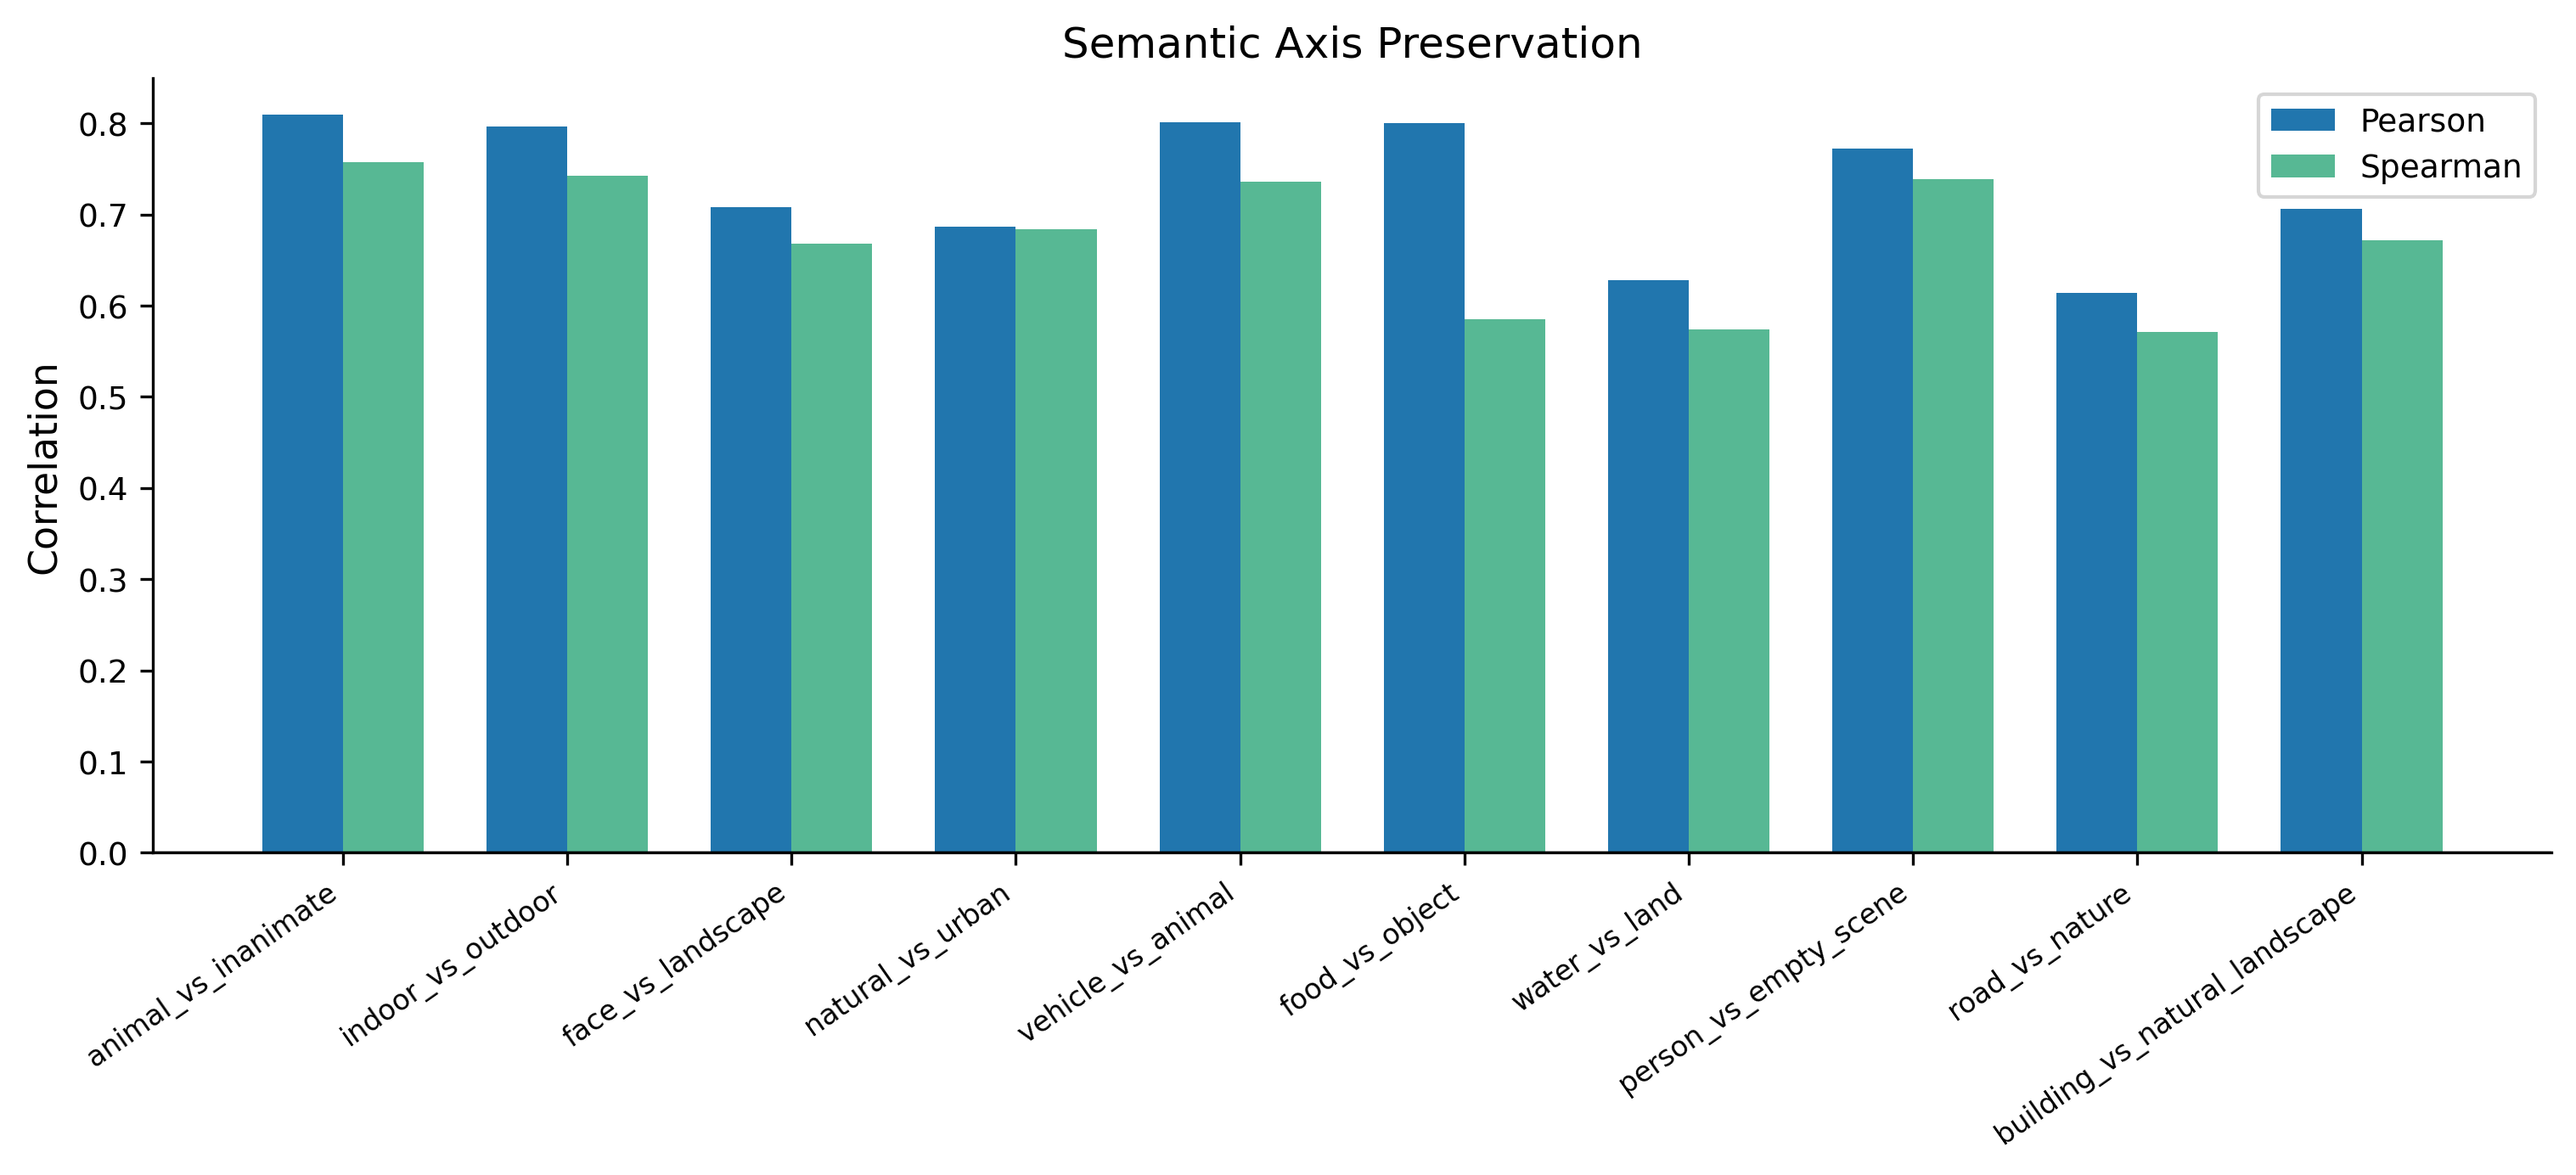
\includegraphics[width=\textwidth]{v62a_semantic_axes_preservation.png}
        \caption{Per-axis Pearson and Spearman correlations of decoded-vs-target projections for the ten interpretable CLIP semantic axes. \emph{Indoor vs.\ outdoor} is the best-preserved axis; \emph{water vs.\ land} is the weakest.}
        \label{fig:v62a_semantic_axes}
    \end{subfigure}

    \caption{Two auxiliary visual probes of the CLS-expert (V62a) SHARED1000 geometry (1000-image gallery), corresponding to two rows of Table~\ref{tab:manifold_evidence}. Both panels characterise the single expert, not the fused system.}
    \label{fig:manifold_evidence_composite}
\end{figure}

\paragraph{What this evidence does and does not say.} The rows of Table~\ref{tab:manifold_evidence} are consistent with a structured fMRI-to-CLIP mapping rather than memorisation: CSLS substantially reduces hubness, local neighbourhoods are preserved well above chance, the representational dissimilarity structure remains positively rank-correlated with the target, and decoded embeddings agree with CLIP text probes on most SHARED1000 trials. Several signals are deliberately not claimed because they are weak or unavailable: vMF-$\kappa$ confidence is near chance on validation and unexported on SHARED1000; manifold-density-only separation between correct and incorrect predictions is rejected in the V62a tests; and reliability-aware selective decoding works on validation but does not transfer to SHARED1000.

\paragraph{Robustness checks.} Three lightweight checks support the primary retrieval result. The V62a SHARED1000 RSA Spearman estimate has a narrow bootstrap interval (width $\approx 0.005$), so the geometric signal is stable rather than outlier-driven. The triple fusion reaches R@5 $= 98.0\%$ and median rank $1$ on SHARED1000, so most non-top-1 errors are near-misses. CSLS gives the same qualitative hubness improvement across all three retrieval spaces (V61a token, V62a 768-D CLS, V66a 768-D ROI), so the correction is a property of the protocol rather than of any single expert. Gallery-size sweeps beyond these artifacts are not performed.

\subsection*{Beyond top-1: semantic axes, interpolation, and counterfactual robustness}
\label{subsec:beyond_top1}

The retrieval and neighbourhood metrics in Table~\ref{tab:manifold_evidence} characterise the V62a expert at a single point on the CLIP manifold. Three additional analyses --- all on the same V62a SHARED1000 protocol --- probe whether the surrounding latent geometry is also semantically organised. The constructs used are operational objects in image-text embedding space, not literal cognitive categories.

\paragraph{Language-space interpretation of decoded embeddings.} Before the three aggregate analyses, Table~\ref{tab:text_probe_examples} shows three representative SHARED1000 cases from the exported semantic-probe artifact, listing the top-three CLIP text concepts for the V62a predicted embedding and for the corresponding ground-truth image embedding under a 29-concept probe library. These per-trial probes are not retrieval outputs; they are a language-space diagnostic for the aggregate agreement@5 of $83.3\%$.

\begin{table}[htbp]
\centering
\scriptsize
\setlength{\tabcolsep}{5pt}
\begin{tabular}{@{}c p{2.9cm} p{2.9cm} p{5.0cm}@{}}
\toprule
\textbf{Sample} & \textbf{Top-3 decoded} & \textbf{Top-3 target} & \textbf{Interpretation} \\
\midrule
$1$ & kitchen; indoor room; food & kitchen; food; indoor room & Top-3 sets coincide; decoded top-1 matches target. \\
$7$ & sports; forest; scene & sports; body; person & Top-1 matches; secondary decoded concepts are scene-context. \\
$8$ & dog; animal; cat & cat; car; animal & Animal class preserved; instance confused (target \emph{cat} in decoded top-3). \\
\bottomrule
\end{tabular}
\caption{Three representative SHARED1000 trials from the CLS-expert (V62a) semantic-probe export, illustrating the range of behaviours behind the aggregate agreement@5 $= 0.833$. These are language-space probes of the decoded embeddings, not retrieval outputs of the fused system.}
\label{tab:text_probe_examples}
\end{table}

\emph{Semantic axes.} Ten interpretable directions are constructed in CLIP text space as
\begin{equation}
    \mathbf{a}_{p \mid q} = \mathbf{t}_p - \mathbf{t}_q,
    \label{eq:semantic_axis}
\end{equation}
where $\mathbf{t}_p,\mathbf{t}_q$ are CLIP text embeddings of paired concepts (e.g.\ \emph{indoor / outdoor}, \emph{animal / inanimate}), covering scene context, semantic category, and object properties. Each predicted V62a embedding is projected onto every axis and compared with the projection of the ground-truth CLIP image embedding. The mean Pearson correlation across axes is $0.732$ and the mean Spearman correlation is $0.673$; \emph{indoor vs.\ outdoor} is the best-preserved axis and \emph{water vs.\ land} is the weakest (Figure~\ref{fig:v62a_semantic_axes}). This is consistent with scene-level distinctions being decoded more reliably than fine compositional ones; the thesis does not attribute axes to specific ROIs.

\emph{Geodesic interpolation on the unit hypersphere.} Twenty pairs of held-out V62a embeddings are interpolated by spherical interpolation, $\mathbf{z}(t) = \mathrm{slerp}(\mathbf{z}_A, \mathbf{z}_B; t)$ for $t \in [0,1]$ in $21$ equally spaced steps. The mean path smoothness (one minus normalised step-to-step displacement) is $0.9998$. Across the $20 \times 21$ steps there are $26$ top-concept transitions in total, distributed gradually along the paths; the stricter \emph{abrupt-transition rate} is only $0.75\%$. The analysed region of CLIP space therefore behaves as a continuous semantic surface locally, not as a discrete cluster lattice; this is not a global topology guarantee.

\emph{Counterfactual semantic editing.} Counterfactual variants $\mathbf{z}^{\text{cf}}_{a,\alpha} = \mathrm{normalize}(\mathbf{z} + \alpha\,\mathbf{a})$ are constructed along the same ten axes. For each of $24$ trials and each axis, the smallest $\alpha$ that flips the dominant text-probe concept is recorded; a finite magnitude exists in every case, with a mean robustness margin of about $0.5$. Decoded embeddings sit in regions where small directed perturbations along language-defined axes shift the dominant semantic label in a controlled way; the margin is descriptive, not a calibrated confidence score.

\emph{What these analyses add.} Where neighbourhood overlap and RSA characterise the order and identity of nearest neighbours, the axis, interpolation, and counterfactual analyses characterise \emph{directions} and \emph{transitions} in the same latent space. All three are V62a-only and do not transfer to the fused system, since the fusion is score-level. We make no claims about perfect manifold reconstruction, region-specific axis attribution, or generative-quality semantic editing.

\section{Qualitative Retrieval Evidence}

The qualitative retrieval panels below show direct triple-fusion top-1 outputs alongside the individual experts, for four representative SHARED1000 stimuli. Each panel displays five columns: the ground-truth stimulus, the V61a-MCTTA16 expert's top-1 retrieval (197\,K-D token space, 16-draw MC-TTA), the V62a expert's top-1 (768-D CLS space), the V66a expert's top-1 (768-D ROI pretrain CLS), and the triple-fusion top-1 after z-scored score-level fusion with CSLS ($k{=}3$, weights $0.7 / 0.1 / 0.2$).

Across all four examples, V61a-MCTTA16 --- the dominant expert at $83.1\%$ CSLS Recall@1 --- retrieves the correct stimulus at rank\,1 on its own. In three of the four cases the weaker experts (V62a at $47.5\%$, V66a at $39.1\%$) miss with semantically plausible but incorrect alternatives; on the fruit-bowl example V66a also retrieves the correct image at rank\,1 while V62a misses only narrowly at rank\,2. In every panel the triple fusion preserves the rank-1 retrieval, illustrating that the frozen score-level combination does not perturb V61a's already-correct results when the weaker experts disagree. These four panels are therefore representative of the $83.1\%$ of SHARED1000 trials in which V61a alone is already correct; the aggregate gain from $83.1\%$ to $86.3\%$ must instead arise on the disjoint subset of trials where V61a's top-1 is wrong, which is not visualised here because per-trial fused ranks across the full benchmark were not exported.

\begin{figure}[p]
    \centering
    \begin{subfigure}[b]{\textwidth}
        \centering
        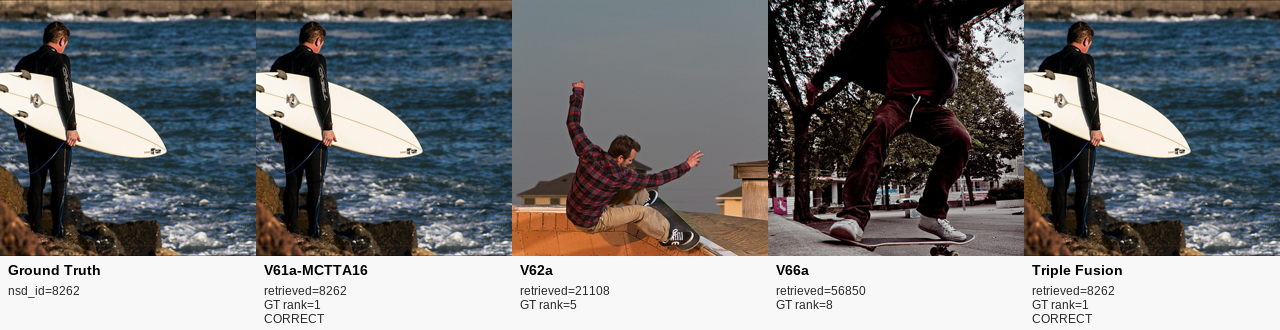
\includegraphics[width=0.93\textwidth]{query_8262.png}
        \caption{Surfer query (NSD\,8262). The two 768-D experts return semantically related but incorrect scenes; V61a-MCTTA16 and the triple fusion both recover the ground truth at rank\,1.}
        \label{fig:query_surfer}
    \end{subfigure}

    \vspace{0.8cm}

    \begin{subfigure}[b]{\textwidth}
        \centering
        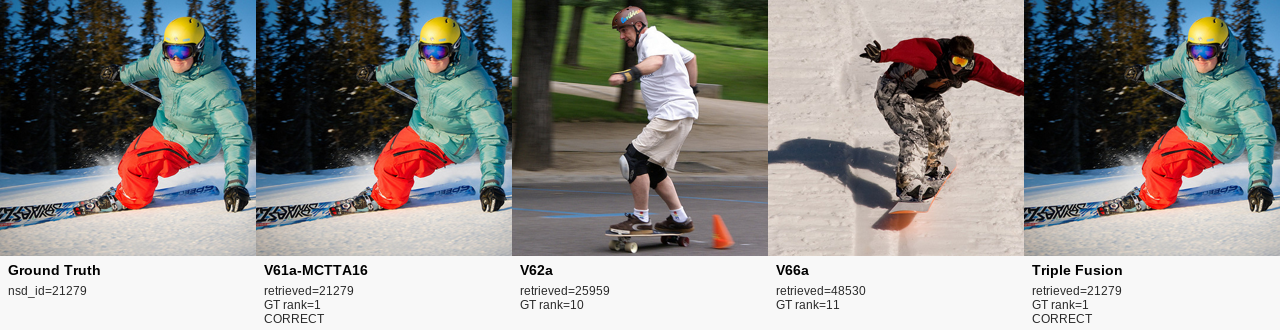
\includegraphics[width=0.93\textwidth]{query_21279.png}
        \caption{Skier query (NSD\,21279). Both 768-D experts miss the correct stimulus by a wide margin; V61a-MCTTA16 and the triple fusion both recover it at rank\,1.}
        \label{fig:query_skier}
    \end{subfigure}

    \caption{Qualitative retrieval successes~(I). Each panel shows, from left to right, the ground-truth stimulus (blue border), the top-1 retrievals of the three individual experts, and the triple-fusion top-1 (dark border). Annotations give the rank of the ground truth for each expert (\checkmark $=$ rank-1, \texttimes\ $=$ miss). The 768-D experts fail with semantically plausible alternatives while the token-space expert with MC-TTA-16 and the fusion recover the exact image at rank~1.}
    \label{fig:retrieval_successes_1}
\end{figure}

\begin{figure}[p]
    \centering
    \begin{subfigure}[b]{\textwidth}
        \centering
        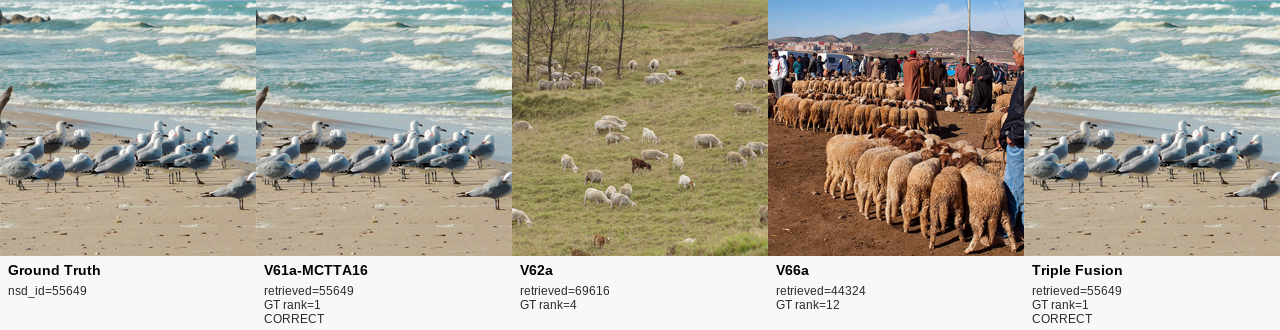
\includegraphics[width=0.93\textwidth]{query_55649.png}
        \caption{Seagull query (NSD\,55649). V62a returns a related but incorrect bird scene, V66a a more distant miss; V61a-MCTTA16 and the triple fusion both recover the ground truth at rank\,1.}
        \label{fig:query_seagulls}
    \end{subfigure}

    \vspace{0.8cm}

    \begin{subfigure}[b]{\textwidth}
        \centering
        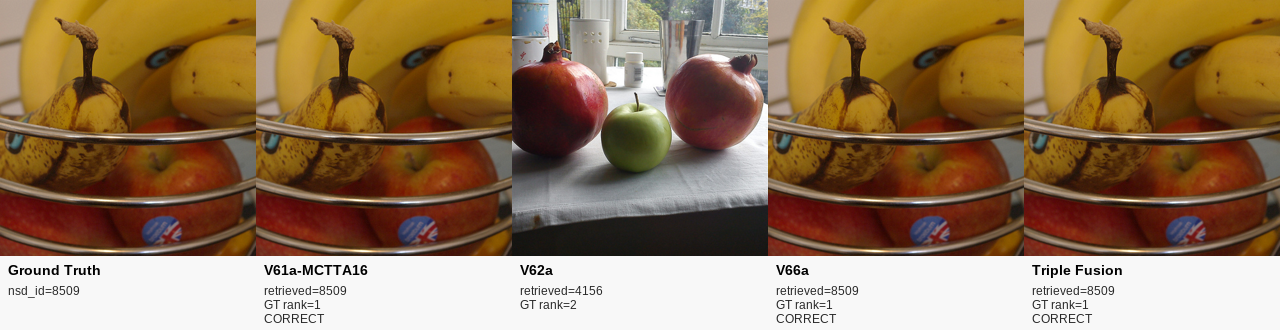
\includegraphics[width=0.93\textwidth]{query_8509.png}
        \caption{Fruit-bowl query (NSD\,8509). V61a-MCTTA16, V66a, and the triple fusion all recover the ground truth at rank\,1; V62a narrowly misses at rank\,2. This convergence among experts is characteristic of the easy regime.}
        \label{fig:query_fruitbowl}
    \end{subfigure}

    \caption{Qualitative retrieval successes~(II). Column order and annotation conventions as in Figure~\ref{fig:retrieval_successes_1}. The seagull example extends the success pattern of the first figure; the fruit-bowl example shows expert convergence where V66a also retrieves the correct image, with V62a a narrow miss at rank\,2.}
    \label{fig:retrieval_successes_2}
\end{figure}

\paragraph{Qualitative error modes.} The four panels in Figures~\ref{fig:retrieval_successes_1} and~\ref{fig:retrieval_successes_2} illustrate two of the typical regimes encountered on SHARED1000: (a) \emph{correct top-1 retrieval} preserved across the fusion (all four panels) and (b) \emph{semantically close but instance-wrong} retrieval at the weaker expert level (V62a / V66a returning a related scene rather than the exact stimulus, e.g.\ a different surfer or skier). Two further error modes that are clearly visible in the aggregate metrics --- (c) trials where V61a is wrong on its own but the fusion recovers the correct image (which must account for at least part of the $+3.2$ percentage-point fusion gain), and (d) trials where all three experts and the fusion fail --- cannot be illustrated here because the corresponding per-trial fused-rank export was not preserved beyond the four illustrated trials. Including paired correction and failure examples once the per-trial fused-rank export is regenerated is a priority for a publication-oriented extension of this work.

\section{Reconstruction Add-on: What the Qualitative Evidence Actually Supports}

The thesis treats reconstruction more conservatively than retrieval. The retrieval system is the primary quantitative contribution, whereas the diffusion add-on is a larger-scale extension evaluated on $n{=}141$ SHARED1000 examples ($n{=}137$ non-perfect) that uses the final triple-fusion top-1 retrievals as the img2img anchor. The pipeline uses Stable Diffusion XL~1.0 (SDXL) with IP-Adapter visual conditioning from the anchor image and the fMRI-predicted CLIP embedding injected into SDXL's native ViT-L/14 text-encoder pathway, generates 16 candidates per example with uncertainty-aware strength derived from a per-example confidence score, and selects the best candidate by CLIP cosine similarity to the predicted embedding. The evidence supplied by the 141-example evaluation supports three conclusions.

First, \emph{exact retrievals should not be harmed}. In the perfect bucket, the final selected output remains identical to the anchor image. This is the correct behaviour: when the retrieval stage is already exact, the generative module should preserve it rather than rewrite it.

Second, \emph{diffusion adds modest but consistent value on non-perfect cases}. Across the good, near-good, and hard buckets, the SDXL with IP-Adapter pipeline improves SSIM, PSNR, and CLIP image similarity while keeping pixel correlation, LPIPS, and AlexNet features essentially flat (Table~\ref{tab:diffusion_summary}, bucketed analysis below). The gains are small in absolute terms, but no bucket shows a regression on any metric, which is a notable change from the earlier SD~2.1 pipeline that exhibited a clear low-level-versus-semantic trade-off.

Third, \emph{SDXL with IP-Adapter conditioning produces modest, non-degrading gains over the retrieval anchor}. The pipeline uses Stable Diffusion XL~1.0 with IP-Adapter cross-attention on the anchor image and injects the fMRI-predicted CLIP embedding into SDXL's native ViT-L/14 text-encoder pathway (the same 768-D space as the decoder output). Strength, guidance, and step count are derived per example from a confidence score $c \in [0,1]$ defined as the CSLS top-1/top-2 margin, mapped linearly to a strength range of $[0,0.30]$. Table~\ref{tab:diffusion_summary} reports modest improvements in SSIM, PSNR, CLIP image similarity, and AlexNet(5)-level identification across $n=141$ SHARED1000 examples ($86.2\%$ 2-way accuracy on the $137$ non-perfect cases), while leaving pixel correlation, LPIPS, and early AlexNet features essentially unchanged. The 2-way AlexNet identification is reported in the same metric family as MindEye and Brain Diffuser but is not protocol-for-protocol comparable, because subject counts, target spaces, and gallery sizes differ. The pipeline conditions on the retrieved top-1 image via IP-Adapter and is therefore anchor-dependent: it should not be interpreted as a pure fMRI-only reconstruction. Retrieval remains the main quantitative contribution.

\begin{table}[htbp]
\centering
\small
\begin{tabularx}{\textwidth}{>{\raggedright\arraybackslash}p{3.4cm} >{\centering\arraybackslash}p{1.6cm} >{\centering\arraybackslash}p{1.6cm} >{\centering\arraybackslash}p{1.6cm} >{\centering\arraybackslash}p{1.6cm} >{\raggedright\arraybackslash}X}
\toprule
\textbf{Metric ($n{=}141$)} & \textbf{Retr.\ mean} & \textbf{Diff.\ mean} & \textbf{$\Delta$ mean} & \textbf{$\Delta$ median} & \textbf{Interpretation} \\
\midrule
Pixel correlation & 0.159 & 0.159 & $-$0.001 & +0.003 & Essentially flat \\
SSIM & 0.202 & 0.214 & +0.012 & +0.015 & Structural similarity improves \\
PSNR (dB) & 9.539 & 9.602 & +0.063 & +0.058 & Consistent improvement; mean and median agree \\
LPIPS $\downarrow$ & 0.657 & 0.657 & $-$0.000 & $-$0.002 & Perceptual distance essentially unchanged \\
CLIP image similarity & 0.744 & 0.750 & +0.005 & +0.009 & SDXL + IP-Adapter preserves semantic similarity \\
AlexNet(2) & 0.467 & 0.466 & $-$0.000 & +0.008 & Early-layer features essentially flat \\
AlexNet(5) & 0.395 & 0.395 & +0.001 & +0.003 & Late-layer features essentially flat \\
\midrule
\multicolumn{6}{l}{\emph{N-way identification accuracy (137 non-perfect examples)}} \\
\midrule
AlexNet(2) 2-way & \multicolumn{2}{c}{75.4\%} & --- & --- & Forced-choice identification (1000 trials) \\
AlexNet(5) 2-way & \multicolumn{2}{c}{86.2\%} & --- & --- & Strong late-layer identification \\
AlexNet(5) 137-way & \multicolumn{2}{c}{19.0\%} & --- & --- & Full-gallery identification (chance: 0.7\%) \\
\bottomrule
\end{tabularx}
\caption{Retrieval-versus-diffusion summary for $n{=}141$ SHARED1000 examples ($n{=}137$ non-perfect) using SDXL~1.0 with IP-Adapter visual conditioning from the anchor and fMRI-predicted CLIP injection (best-of-16, uncertainty-aware strength). PSNR is computed over the $137$ non-perfect examples. The bottom rows report $n$-way AlexNet identification: the reconstruction's feature vector must rank the correct ground truth above $n{-}1$ distractors. This is reported in the same metric family as MindEye and MindEye2 but is not protocol-for-protocol comparable.}
\label{tab:diffusion_summary}
\end{table}

The bucketed analysis refines the picture. Perfect cases ($n=4$) remain perfect, validating the anchor-first controller. The good ($n=117$), near-good ($n=13$), and hard ($n=7$) buckets each show modest gains in SSIM, PSNR, and CLIP image similarity, with pixel correlation and AlexNet features essentially flat. No bucket shows a metric regression of the kind observed with the earlier SD~2.1 pipeline. This pattern is attributable to two changes relative to the previous pipeline: SDXL's stronger image prior generates higher-fidelity textures, and IP-Adapter cross-attention provides a principled visual conditioning pathway that does not conflict with the semantic CLIP injection. The evaluation on $n=137$ non-perfect examples makes these conclusions statistically more defensible than the earlier $n=12$ non-perfect subset, where outlier-driven mean--median divergence obscured the signal; we still treat the gains as \emph{modest and non-degrading} rather than as evidence of a large reconstruction win, in line with the conservative framing of this section.

\begin{sidewaysfigure}[p]
    \centering
    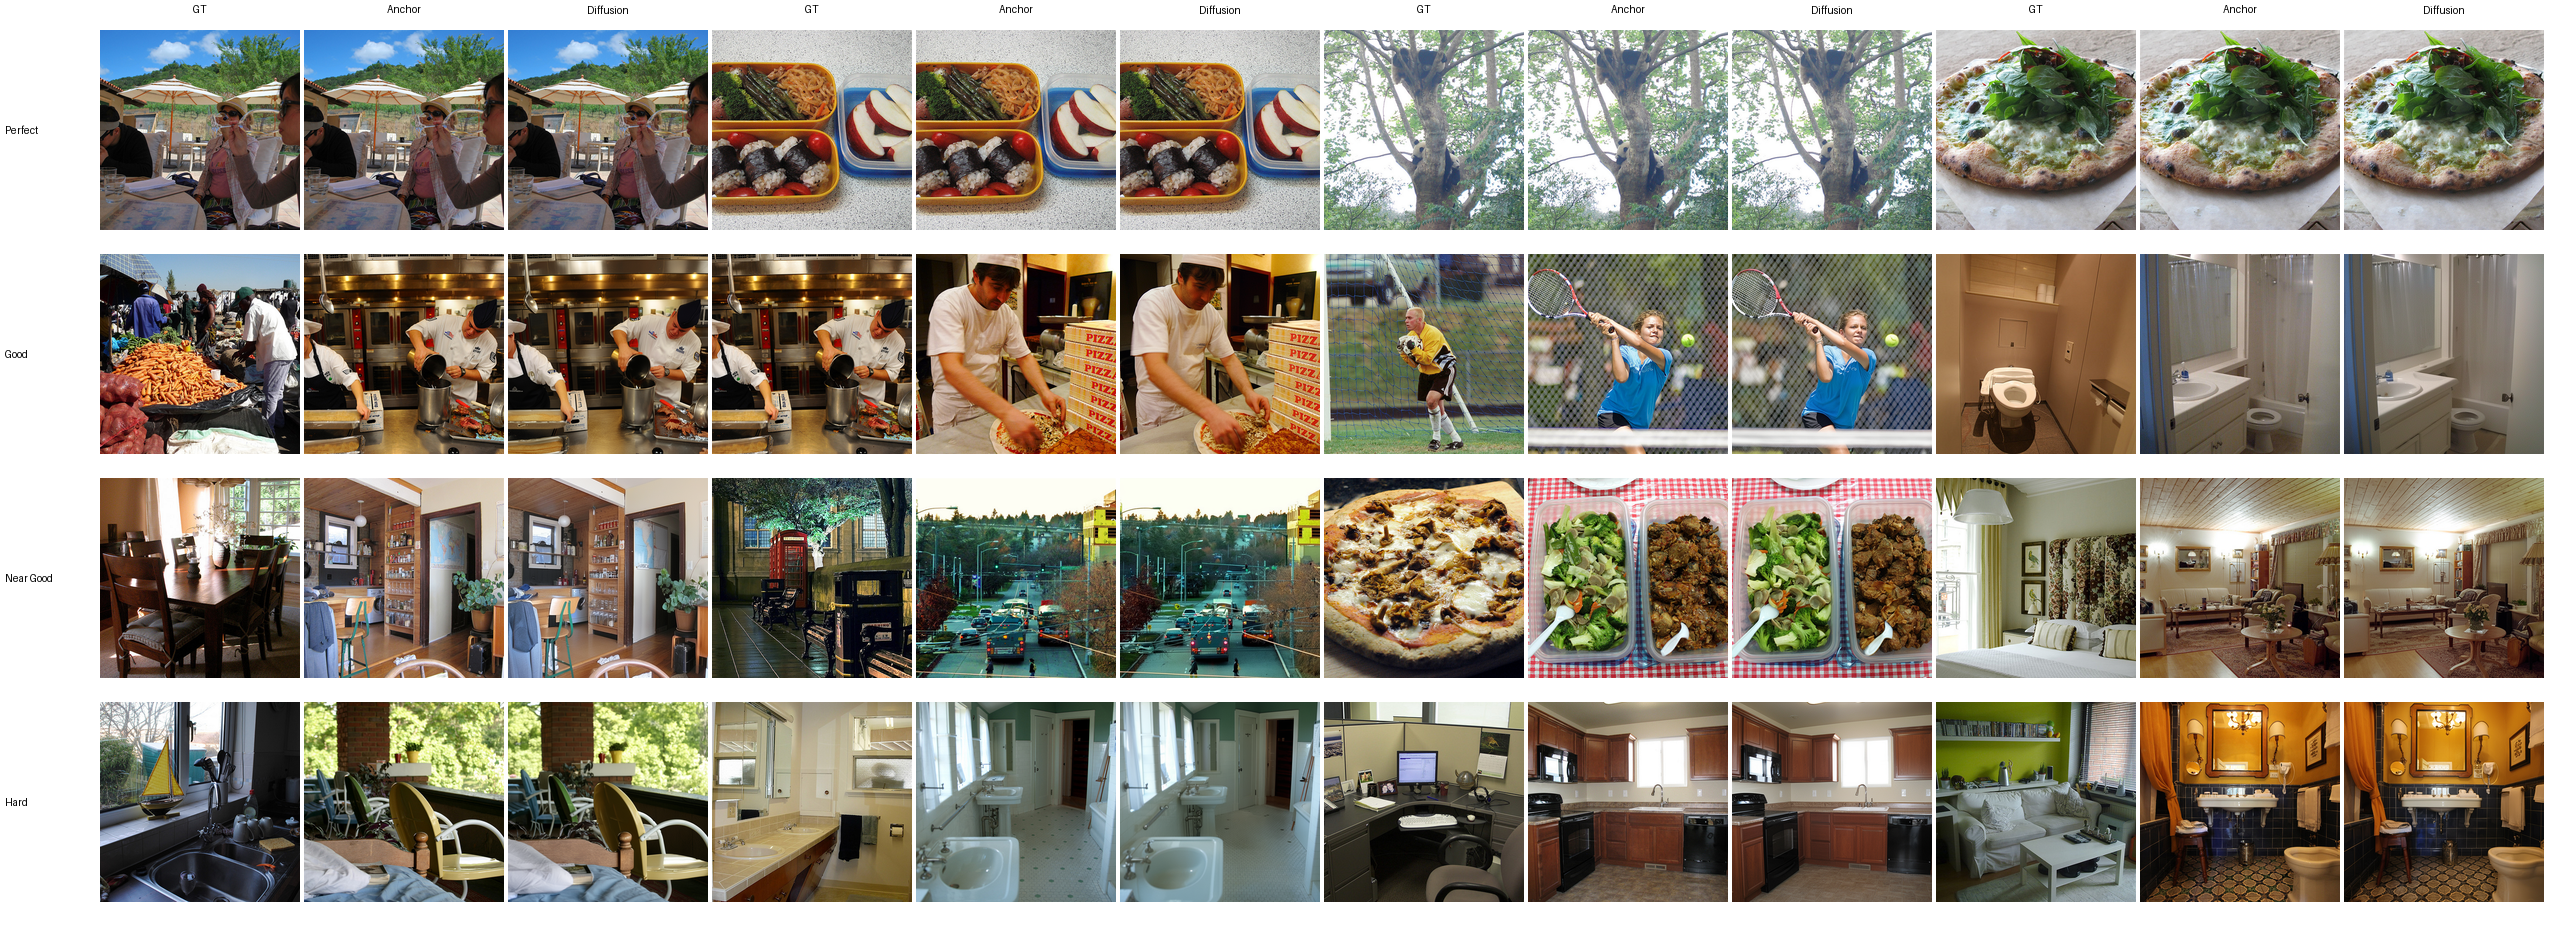
\includegraphics[width=0.95\textheight]{reconstruction_examples_composite.png}
    \caption{Representative SDXL + IP-Adapter reconstruction examples anchored on the triple-fusion top-1 retrievals (rotated so the per-tile labels remain readable at print size). \textbf{Rows} correspond to the four difficulty buckets: \emph{Perfect} (identity pass-through), \emph{Good}, \emph{Near Good}, \emph{Hard}. \textbf{Columns} form two side-by-side triplets of \emph{Ground truth}, \emph{Anchor} (triple-fusion top-1), and \emph{Diffusion} (SDXL conditioned on the anchor and on the fMRI-predicted CLIP embedding, best-of-$16$, uncertainty-aware strength). The diffusion stage produces modest improvements on the aggregate metrics of Table~\ref{tab:diffusion_summary}; because every reconstruction conditions on the retrieved top-1 image, these outputs are anchor-dependent and not pure fMRI-only reconstructions.}
    \label{fig:reconstruction_examples}
\end{sidewaysfigure}

\section{Ablation-Oriented Discussion}

Although the revised thesis now reports the frozen cross-architecture triple fusion as the final exported retrieval system, with the V35 plus N1v28a fixed fusion retained as a methodological milestone, the negative results remain almost as informative as the positive ones. Several experimentally attractive ideas did not produce the expected gains:
\begin{itemize}
    \item purely probabilistic directional formulations proved harder to stabilize than initially expected;
    \item richer latent targets improved pointwise expressivity but sometimes degraded retrieval geometry;
    \item anatomically structured or tokenized formulations were not automatically superior to strong full-vector baselines;
    \item learned global gates and residual rerankers easily overfit if expert disagreement patterns are not matched across train and evaluation conditions;
    \item the earlier SD~2.1 reconstruction pipeline with empty-prompt or text-encoder-injected CLIP conditioning produced a clear low-level-versus-semantic trade-off, regressing on SSIM, LPIPS, and CLIP image similarity on a preliminary 16-example diagnostic subset; replacing it with SDXL~1.0 plus IP-Adapter visual conditioning and scaling to $141$ examples removed those regressions and yielded the modest non-degrading gains reported in Table~\ref{tab:diffusion_summary}.
\end{itemize}

This ablation-oriented perspective is valuable because it prevents over-interpretation. Instead of claiming that every added modelling idea is useful, the thesis distinguishes between improvements that genuinely change the retrieval outcome and changes that are aesthetically appealing but practically weak under the current data regime.

\section{Comparison to the Literature}

The results of the thesis should be interpreted in context rather than in isolation. Recent large-scale systems show that much larger gains are possible when one combines stronger shared-subject scaling, richer token targets, and more ambitious alignment strategies \cite{Scotti2024}. The present thesis does not aim at parity with those systems; it answers a narrower question, namely how the available information should be decomposed and fused within a retrieval-focused single-subject decoding setting.

In that narrower setting, the thesis supports three claims. First, compact retrieval, shortlist-local reranking, and rich regression are better treated as distinct roles than forced into one universal latent space. Second, once a strong compact expert exists, complementary frozen score-level fusion can still deliver substantial gains without retraining, as the V35 plus N1v28a milestone illustrates. Third, additional gains remain available by extending the same frozen-fusion idea across target spaces and architecture families together with single-model strengthening through MC-TTA. The final $86.3\%$ CSLS Recall@1 on SHARED1000 is therefore not just a higher number; it is evidence that, in this setting, retrieval quality depends as much on how information is combined at inference time as on how it is first predicted. Numerical comparisons to large-scale literature systems remain contextual at the metric-definition level, not protocol-for-protocol, because galleries, splits, and CLIP backbones often differ.

\begin{table}[htbp]
\centering
\footnotesize
\begin{tabularx}{\textwidth}{>{\raggedright\arraybackslash}p{2.5cm} >{\raggedright\arraybackslash}p{1.6cm} >{\raggedright\arraybackslash}p{2.3cm} >{\raggedright\arraybackslash}p{2.2cm} >{\raggedright\arraybackslash}X}
\toprule
\textbf{Work} & \textbf{Dataset} & \textbf{Subject setting} & \textbf{Main focus} & \textbf{Relation to this thesis} \\
\midrule
Allen et al. \cite{Allen2022} & NSD release & 8 subjects & 7T NSD data resource & Provides the data, splits, and SHARED1000 benchmark used throughout this thesis \\
Takagi and Nishimoto \cite{Takagi2023} & NSD & per-subject & Stable-Diffusion-based reconstruction & Earlier reconstruction-first design; this thesis is retrieval-first and uses CLIP-aligned latents \\
Ozcelik and VanRullen \cite{Ozcelik2023} & NSD & per-subject & Latent-diffusion reconstruction (Brain Diffuser) & Closest reconstruction-pipeline precedent; informs the SDXL + IP-Adapter add-on here \\
MindEye \cite{Scotti2023} & NSD & per-subject & CLIP-target retrieval + diffusion reconstruction & Inspires the retrieval-first framing; this thesis reuses the same MindEye-style AlexNet $n$-way identification metric \\
MindEye2 \cite{Scotti2024} & NSD & shared-subject scaling & Multi-subject pretraining + image reconstruction & Strongest large-scale precedent; the present thesis does not match its multi-subject scale and does not claim parity \\
\textbf{This thesis} & NSD, subj01 only & single-subject & Retrieval-first frozen score-level fusion + auxiliary diffusion add-on & Headline endpoint is $86.3\%$ CSLS R@1 on SHARED1000 (Table~\ref{tab:final_results}); reconstruction is reported on $141$ examples with $86.2\%$ 2-way AlexNet(5) identification (Table~\ref{tab:diffusion_summary}) \\
\bottomrule
\end{tabularx}
\caption{Contextual comparison to representative fMRI-to-image decoding work. Subject counts, target spaces, gallery sizes, and reconstruction protocols differ across studies; the metrics are reported in the same metric family but absolute values are not protocol-for-protocol comparable without re-running each system under a shared protocol.}
\label{tab:literature_comparison}
\end{table}

\section{Ethical Considerations and Scope of Brain Decoding}
\label{sec:ethics}

The scope of this thesis is deliberately narrow. The decoder is trained and evaluated on the Natural Scenes Dataset \cite{Allen2022}, in which volunteer subjects view known external natural images under controlled laboratory conditions and with prior informed consent. The decoder maps the resulting fMRI responses to image-aligned CLIP embeddings of those external stimuli; it does not infer private thoughts, intentions, memories, or imagined content, and it is not a general "mind reading" system. The final retrieval endpoint is meaningful only against a fixed pre-specified gallery, the reconstruction add-on is meaningful only when conditioned on a retrieved anchor image, and every stage depends on subject-specific fMRI preprocessing, voxel selection, and per-session normalisation. None of these conditions are met in any ecological setting outside the laboratory protocol.

The methodology is therefore appropriate to discuss as a step toward more reliable perception-decoding tools for neuroscience research and for assistive or medical use cases that involve informed consent, but it would be inappropriate to extrapolate from it to claims about decoding mental states in the wild. Future systems that approach more general decoding regimes will require explicit attention to subject consent, neural-data privacy, dataset governance, model misuse risks (including unauthorised inference from passively collected scans), and clear communication to non-technical audiences about what such systems can and cannot do.

\section{Limitations}

Despite the encouraging results, several limitations remain. The study is still constrained by subject scale, by the difficulty of cross-subject alignment, and by the fact that retrieval is quantitatively emphasized more strongly than reconstruction fidelity. The final best system also relies on a frozen inference-time score fusion rather than on a fully end-to-end fusion-aware training objective. The use of 16-draw MC-TTA on the dominant 197K expert increases inference cost relative to a single forward pass. Validation Recall@1 in the V60--V66 experiment family can be inflated by shared-image overlap with pretraining splits, which is why SHARED1000 CSLS Recall@1 is treated as the primary SHARED1000 benchmark endpoint throughout this chapter. The diffusion add-on is evaluated on $n{=}141$ SHARED1000 examples ($n{=}137$ non-perfect), which provides statistical defensibility for the aggregate conclusions but still covers only the SHARED1000 gallery; its performance on different galleries or subjects is not assessed.

These limitations do not weaken the current conclusions; rather, they clarify the next research steps. The thesis has reached a point where the main challenge is no longer basic pipeline validity, but how to preserve complementary expert signals while scaling toward stronger shared-subject and reconstruction-aware systems.

\paragraph{Reconstruction-side ablation plan.} A more complete reconstruction study should isolate the contribution of the retrieved image anchor from the contribution of the predicted fMRI-derived CLIP signal. This requires running the same pipeline under five controlled conditions: (i) anchor-only generation with no CLIP injection, (ii) anchor plus predicted-CLIP injection (the current configuration), (iii) an incorrect-anchor control in which the IP-Adapter image is replaced by an unrelated SHARED1000 image while the predicted CLIP is retained, (iv) CLIP-only conditioning with no anchor image at all, and (v) a ground-truth-anchor upper bound in which the IP-Adapter receives the true stimulus image. The current thesis does not include this 5-way ablation grid; it is identified as the priority experiment for a future extended study because only that comparison disentangles \emph{how much} of the reported reconstruction quality is carried by the retrieval anchor and \emph{how much} by the fMRI-predicted latent signal.

\section{Summary of Claims, Evidence, and Scope}
\label{sec:claim_register}

Table~\ref{tab:defense_summary} consolidates the main lines of evidence in this thesis. Each row pairs a thesis-level claim with the in-thesis evidence and the scope under which the claim is defended; repository-level artifacts are in Table~\ref{tab:artifact_map}.

\begin{table}[htbp]
\centering
\footnotesize
\begin{tabularx}{\textwidth}{@{}>{\raggedright\arraybackslash}p{2.6cm} >{\raggedright\arraybackslash}X >{\raggedright\arraybackslash}p{3.0cm} >{\raggedright\arraybackslash}X@{}}
\toprule
\textbf{Claim} & \textbf{What the thesis demonstrates} & \textbf{Evidence} & \textbf{Scope / limitation} \\
\midrule
Retrieval (primary) & Frozen score-level fusion of three independently trained experts reaches $86.3\%$ CSLS R@1 on SHARED1000. & Tables~\ref{tab:final_results},~\ref{tab:expert_complementarity} & subj01 only; per-trial fused ranks not exported $\Rightarrow$ no bootstrap CI. \\
CSLS + complementarity & CSLS substantially reduces hubness on the analysed expert; the fusion gain exceeds redundant-ensembling expectation. & Table~\ref{tab:manifold_evidence}, \S\ref{sec:why_triple_fusion_anchor} & Manifold evidence is V62a-only; complementarity claim is aggregate. \\
Reconstruction add-on & SDXL + IP-Adapter + fMRI-predicted CLIP yields modest, non-degrading gains in SSIM, PSNR, CLIP-I, AlexNet(5) on 141 SHARED1000 examples. & Table~\ref{tab:diffusion_summary} & Anchor-dependent; 5-way anchor-vs-CLIP ablation not run. \\
Methodological design & Compact / rerank / rich decomposition and frozen score-level fusion are scientifically distinct contributions, validated under a shared protocol. & Tables~\ref{tab:final_results},~\ref{tab:experimental_waves}; \S\ref{sec:architecture_evolution} & Single-subject evaluation; not a multi-subject claim. \\
Ethical scope & The system decodes viewed external stimuli from consenting NSD subjects against a fixed gallery; it is not a general ``mind reading'' system. & \S\ref{sec:ethics} & Does not extrapolate to ecological settings, mental imagery, or non-consensual inference. \\
\bottomrule
\end{tabularx}
\caption{Summary of claims, evidence, and scope.}
\label{tab:defense_summary}
\end{table}


\chapter{Conclusions and Future Work}
\label{chap:conclusions}

This thesis studied neural decoding of visual perception from fMRI using CLIP-guided latent targets and retrieval-oriented modelling, treating the problem not as a regression task but as a structured mapping from cortical activity to a visual representation space that supports both retrieval and downstream generation. The work emphasises model design and scientific debugging in equal measure, since the validity of any reported result depends on the integrity of preprocessing, target caching, training, and evaluation.

The final outcome integrates three levels of insight. Architecturally, the project converges on a multi-head decoder that separates compact shortlist retrieval, shortlist-local reranking, and rich latent regression. At the single-model level, the strongest expert is strengthened by Monte Carlo test-time augmentation on a token-space target at $16\times$ inference compute. At the system level, a frozen cross-architecture score-level fusion combines this MC-TTA expert with two complementary 768-D experts and reaches $86.3\%$ CSLS Recall@1 on SHARED1000; the earlier V35 plus N1v28a fixed fusion at $77.2\%$ remains an important methodological milestone. The fusion operates at score level rather than as an end-to-end fusion-trained architecture, and therefore improves retrieval without producing a unified fused latent embedding.

The most important scientific outcome is interpretive clarity. The thesis does not claim to solve the problem or to match the strongest large-scale shared-subject methods; instead, it narrows the remaining gap. Early obstacles came from concrete bugs and unstable optimisation; once those were eliminated, the dominant limitations became structural --- subject scale, alignment, and the geometry of high-dimensional retrieval spaces. Documenting the modelling ideas that failed in practice reduces the future search space and distinguishes cosmetic from genuinely effective design choices.

\paragraph{Future work.} Four directions stand out as the strongest immediate extensions:
\begin{itemize}
    \item per-trial fused-rank export across SHARED1000, with bootstrap $95\%$ confidence intervals on Recall@1, Recall@5, and MRR, and a paired correct-vs-wrong transition analysis between the strongest single expert and the fusion;
    \item a 5-way reconstruction ablation that isolates the contribution of the retrieval anchor from the contribution of the predicted CLIP signal (anchor-only, anchor + predicted CLIP, wrong-anchor control, CLIP-only, ground-truth-anchor upper bound);
    \item a fusion-weight / CSLS-$k$ / MC-TTA-depth ablation grid on SHARED1000, replacing the current single-recipe report with a calibration sweep;
    \item an optional multi-subject extension that integrates shared-subject learning and functional alignment in the spirit of MindEye2 \cite{Scotti2024}.
\end{itemize}

The main takeaway of the thesis is methodological. In the evaluated single-subject setting, compact shortlist retrieval, shortlist-local reranking, and rich latent regression are best treated as distinct roles, and complementary experts can still be combined profitably after training through frozen score-level fusion. The final system reaches $86.3\%$ CSLS Recall@1 on the held-out SHARED1000 benchmark and therefore establishes a strong, reproducible retrieval result under a clearly specified protocol. The SDXL + IP-Adapter add-on is useful as a secondary qualitative extension, but it remains anchor-dependent and should not displace retrieval as the central contribution. The most defensible claim of the thesis is therefore not that it solves fMRI-to-image decoding in general, but that it delivers a rigorous retrieval-first framework whose gains are interpretable, reproducible, and suitable for a stronger conference-oriented extension.

\begin{figure}[htbp]
    \centering
    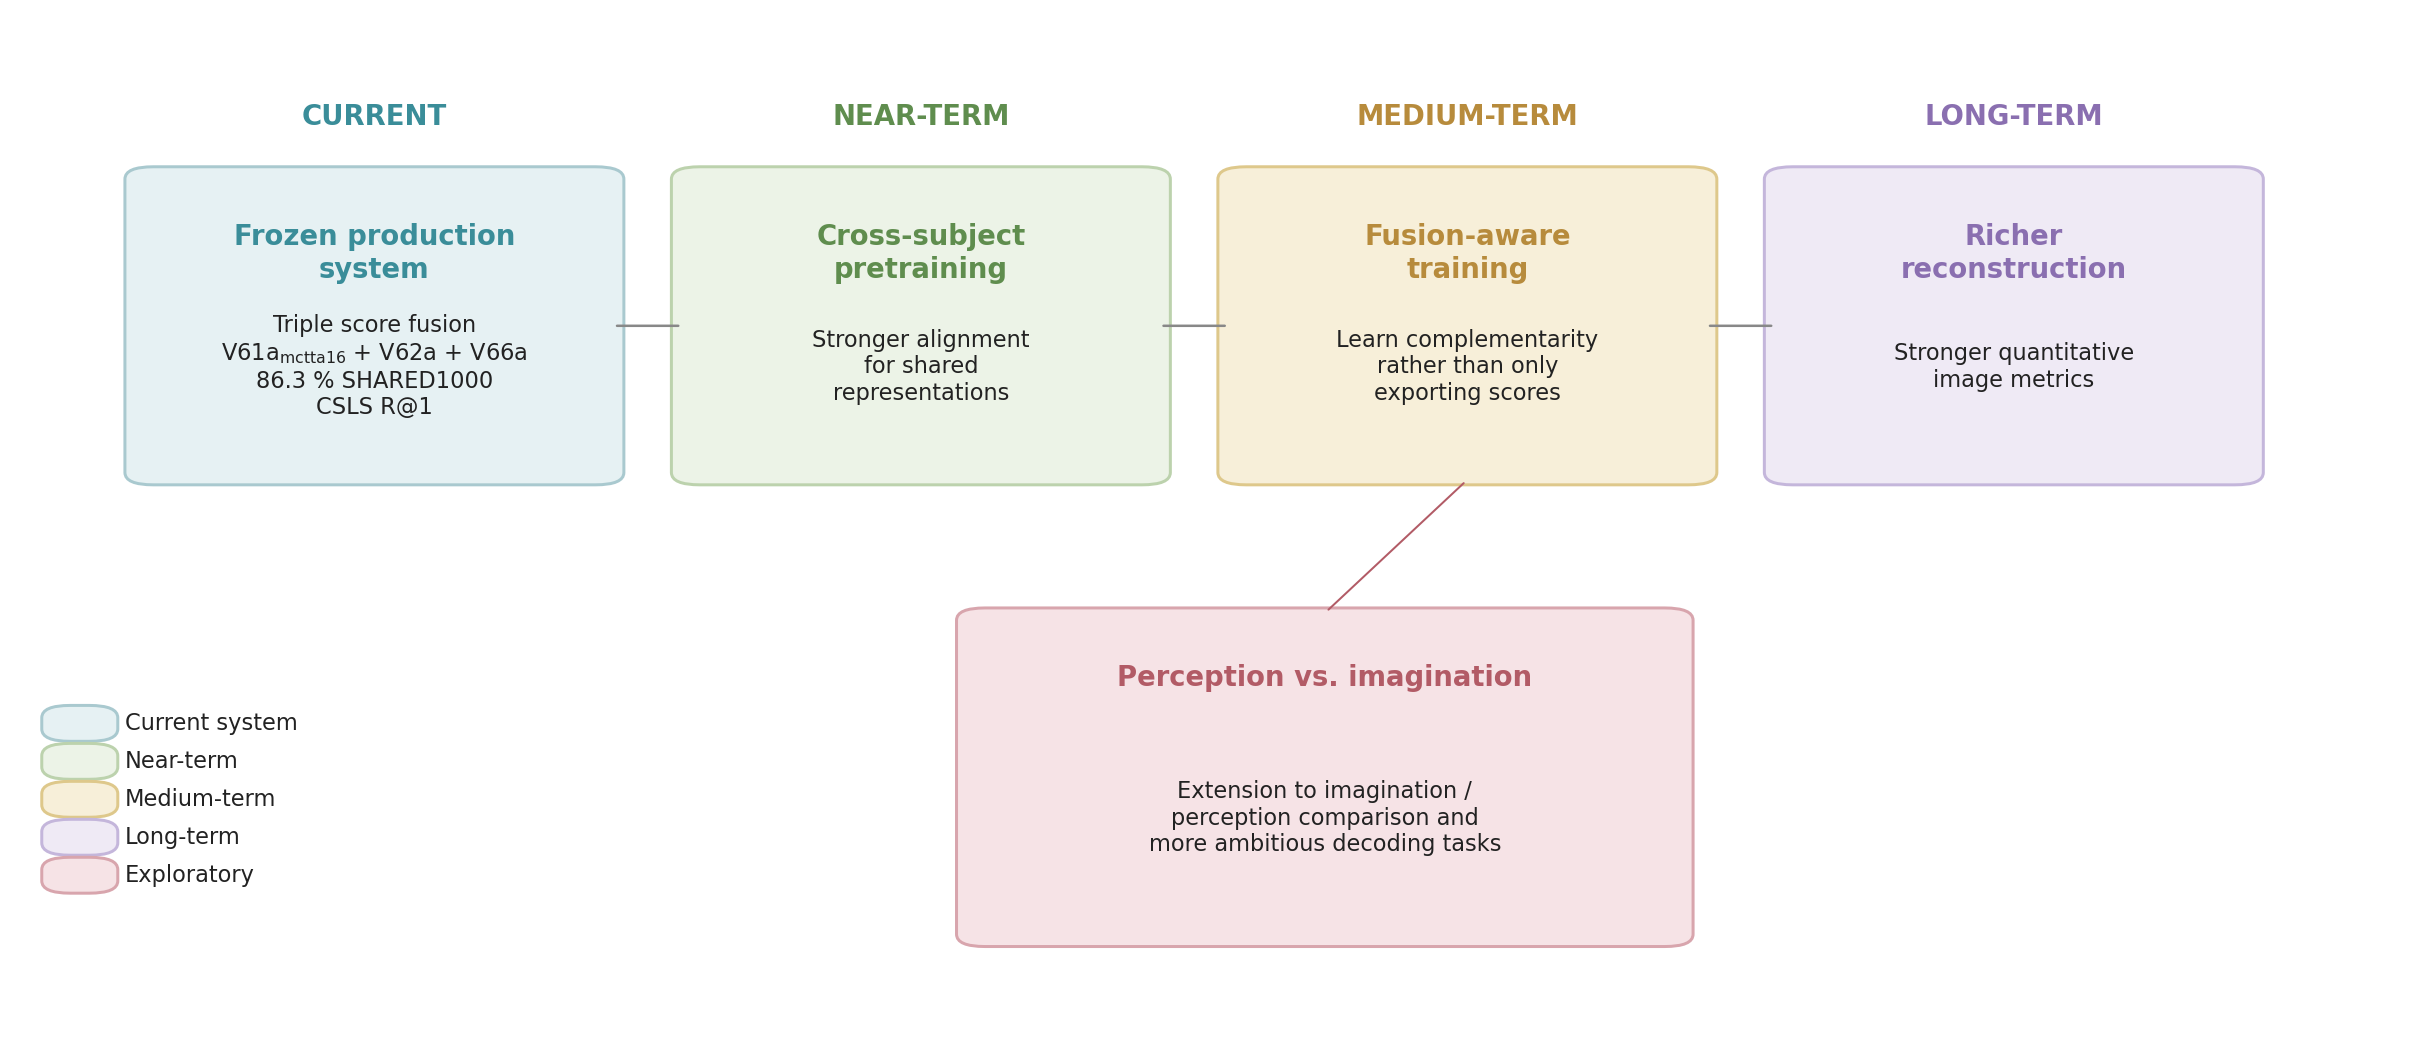
\includegraphics[width=\textwidth]{future_roadmap.png}
    \caption{Roadmap after the final triple-fusion retrieval system: stronger shared-subject alignment, fusion-aware training, more rigorous reconstruction evaluation, and broader perception-versus-imagery decoding.}
    \label{fig:future_roadmap}
\end{figure}


\bibliographystyle{plain}
\bibliography{references}

\end{document}
